\section{Proofs}
\subsection{Proof of Theorem \ref{remark_1}}
\begin{proof}
Let $\pi^*$ be any optimal policy (possibly history-dependent). Suppose $\pi^*$ prescribes different action distributions at the same state $s$ depending on the history that led to $s$.

Let $\delta_1$ and $\delta_2$ be two such distributions with $\EE_{a\sim\delta_1} Q^*(s, a) > \EE_{a\sim\delta_2} Q^*(s, a)$, where $Q^*$ is the optimal value in RL. Then construct $\pi'$ that behaves like $\pi^*$ everywhere except it always uses $\delta_1$ whenever the state is $s$ (ignoring history). The future trajectories from any visit to $s$ are stochastically identical under $\pi^*$ and $\pi'$, except that $\pi'$ gets strictly higher expected return from every time $s$ is visited after histories that would have triggered $\delta_2$ under $\pi^*$.

Thus, $V^{\pi'}(s_0) > V^{\pi^*}(s_0)$ for some state, contradicting optimality of $\pi^*$. Therefore, this optimal policy must prescribe the same action distribution at state $s$ regardless of history. In other words, there exists an optimal Markovian policy. In the following, we will prove by contradiction that policies that exhibit reflective exploration cannot be Markovian.

Assume $\pi$ is a Markovian policy. Then there exists a mapping $\mu : \mathcal{S} \to \Delta(\mathcal{A})$ such that, for every history $h_t$, $\pi(\cdot \mid h_t) = \mu(\cdot \mid s(h_t))$. Define the process $X_t := s(h_t)$ and set $\upsilon := \mu$. By construction, $\pi(\cdot \mid h_t) = \upsilon(\cdot \mid X_t)$ for all $t$.

According to Definition \ref{def:reflective}, there is a measurable $\psi$ such that $X_t = \psi(\varphi(s_t))$ and thus $s(h_t) = \psi(\varphi(s(h_t)))$. Let $s,s'$ be reachable states and $\varphi(s) = \varphi(s')$. Then $s =\psi(\varphi(s)) = \psi(\varphi(s')) = s'$.

Therefore, there exist $t_1 > t_2$ and histories $h_{t_1}, h_{t_2}$ such that
\$
\varphi(s(h_{t_1})) = \varphi(s(h_{t_2})), 
\qquad 
\pi(\cdot \mid h_{t_1}) \neq \pi(\cdot \mid h_{t_2}).
\$

Thus, we obtain $s(h_{t_1}) = s(h_{t_2}) =: s_*$. But then, using the Markov property of $\pi$, we have $\pi(\cdot \mid h_{t_1}) = \mu(\cdot \mid s_*) = \pi(\cdot \mid h_{t_2})$, which contradicts $\pi(\cdot \mid h_{t_1}) \neq \pi(\cdot \mid h_{t_2})$. Therefore, $\pi$ is not Markovian.
\end{proof}

\subsection{Proof of Theorem \ref{thm_ada}}
Before the proof, we first provide several useful definitions and lemmas.
\begin{definition}[Epistemic POMDP]
We define the \emph{epistemic POMDP} $\mathcal{P} \coloneqq(\mathcal{Z}, \mathcal{O}, \mathcal{A}, P, r, \rho)$ where the hidden state space as $\mathcal{Z} \coloneqq \mathcal{S} \times \mathcal{M}$, with state $z_t = (s_t,M)$; action space $\mathcal{A}$; observation space $\mathcal{O} \coloneqq \mathcal{S}$ with an observation map $O((s,M)) = s$; transition kernel $P\bigl((s_{t+1},M') \mid (s_t,M), a_t\bigr)=\mathbf{1}\{M' = M\} \, P_M(s_{t+1} \mid s_t,a_t)$; reward $r((s,M),a) = r_M(s,a)$; and initial state distribution $\rho((s_0,M)) \coloneqq p(M \mid D)\,\rho_M(s_0)$, where $\rho_M$ is the initial-state distribution in $M$. For a policy $\pi$, let $J_{\mathcal{P}}(\pi)$ denote its expected return in this POMDP.
\end{definition}

\begin{lemma}[Equivalence of Objectives]
\label{lem:epistemic-equivalence}
For any policy $\pi$, $\pi$ is Bayes-optimal if and only if it is optimal for the epistemic POMDP $\mathcal{P}$, i.e., 
\$
J_{\mathcal{P}}(\pi) \;=\; J_{\mathrm{Bayes}}(\pi).
\$
\end{lemma}

\begin{proof}
By construction of the initial distribution,
\$
(s_0,M) \sim \rho\quad\Longleftrightarrow\quad M \sim p(M \mid D),\; s_0 \sim \rho_M.
\$
Conditioned on $M$, the state transitions and rewards in $\mathcal{P}$ coincide exactly with those of the MDP $M$ under policy $\pi$, and the observation $o_t = s_t$ carries no additional information beyond $s_t$. Thus,
\$
J_{\mathcal{P}}(\pi) = \mathbb{E}_{M \sim p(M \mid D)}[J_M(\pi)] = J_{\mathrm{Bayes}}(\pi),
\$
which proves the claim. Similar results are also presented in \cite{singh1994learning,duff2002optimal}.
\end{proof}

Now we are ready to prove Theorem \ref{thm_ada}.
\begin{proof}[Proof of Theorem \ref{thm_ada}]
By Lemma~\ref{lem:epistemic-equivalence}, Bayes-optimal policies coincide with optimal
policies for the epistemic POMDP $\mathcal{P}$.

It is a standard result in POMDP theory that there exists an optimal policy that is a function only of the belief state $\beta_t$, where
\$
\beta_t(z) \coloneqq \mathbb{P}(z_t = z \mid h_t, D).
\$
Thus there exists a policy $\pi^\star$ and a measurable mapping $\tilde{\mu}^\star$ such
that
\$
\pi^\star(a_t \mid h_t) = \tilde{\mu}^\star(a_t \mid \beta_t).
\$
In the epistemic POMDP, the hidden state is $z_t = (s_t,M)$ and the observation is
$o_t = s_t$. Therefore, the belief factors as
\$
\beta_t(s,M) = \mathbf{1}\{s = s_t\} \, p(M \mid h_t, D),
\$
so $\beta_t$ is uniquely determined by the pair $(s_t, p(\cdot | h_t, D))$.
Since the offline posterior $p(M | D)$ is fixed, the mapping $b(h_t)(M)$ is in one-to-one correspondence with $p(M | h_t, D)$, and hence with $\beta_t$.
Thus there exists a measurable function $\mu^\star$ such that for all $h_t$,
\$
\tilde{\mu}^*(a_t \mid \beta_t) = \mu^\star(a_t \mid s_t, b(h_t)).
\$
Therefore, we obtain
\$
\pi^\star(a_t \mid h_t) = \tilde{\mu}^\star(a_t \mid \beta_t) = \mu^\star(a_t \mid s_t, b(h_t)),
\$
so $\pi^*$ is uncertainty-adaptive.
Since $\pi^*$ is optimal for $\mathcal{P}$, it is Bayes-optimal for
$J_{\mathrm{Bayes}}$ by Lemma~\ref{lem:epistemic-equivalence}, completing the proof.
\end{proof}


\subsection{Proof of Theorem \ref{thm_exp}}
\begin{proof}
Consider a full binary decision structure of depth $T^*$, with leaf set $\mathcal{L}$ of size $|\mathcal{L}|=2^{T^*}$. The states are the tree nodes, with the initial state fixed as the root node. The actions include the moves from the parent nodes to the child nodes as well as a resetting action from the leaf node to the root node. The rewards are not known and differ in different MDP hypotheses. Specifically, the reward is defined as $r_{\mathcal{M}_i}(s) = \mathbbm{1}(s = s_i)$, where $s_i$ is a unique leaf node for $\mathcal{M}_i$. The prior of MDPs is $p(\mathcal{M}_i)= 1/|\mathcal{L}|$, where $i=1,\cdots, |\mathcal{L}|$. The cumulative return is undiscounted with the minimum traverse steps as the horizon $T$. The episode terminates once the agent receives a $1$ reward.

For any Markovian policy $\pi$, define $f(s) = p(\exists t\geq0:s_t=s\mid \pi)$. We define $p_s$ as the probability that $\pi$ goes left at an internal node $s$. By the Markov property, for any left and right children $s_L$ and $s_R$ of node $s$, it holds that $f(s_L) = f(s) p_s$ and $f(s_R) = f(s) (1-p_s)$. Thus, $f(s_L) + f(s_R) = f(s)$. By a simple induction on depth, it follows that at every depth $d$, $\sum_{s:\text{depth}(s)=d} f(s)= 1$. In particular, $\sum_{l\in\mathcal{L}}f(l) = 1$. Since the total return under $\mathcal{M}_i$ is $V(\pi\mid \mathcal{M}_i) = p(\pi\text{ ends at leaf }l_i) = f(l_i)$, the expected return for the optimal Markovian policy is
\$
\frac{1}{|\mathcal{L}|}\sum_{i=1}^{|\mathcal{L}|}V(\pi\mid \mathcal{M}_i) = \frac{1}{2^{T^*}}\sum_{l\in\mathcal{L}}f(l) = \frac{1}{2^{T^*}}.
\$

We construct the uncertainty-adaptive policy as follows. Let $\mathcal{C}= \{\mathcal{M}_1,\dots,\mathcal{M}_{|\mathcal{L}|}\}$ be the set of models that are still consistent with the observed rewards in $h_t$.
When the agent visits a leaf $s$ and observes reward $r \in \{0,1\}$,
we update $\mathcal{C}\leftarrow\{\mathcal{M} \in \mathcal{C}: r_{\mathcal{M}}(s) = r\}$. For each $i$, there is exactly one leaf $s$ with $r_{\mathcal{M}_i}(s) = 1$. Hence, under any true MDP $\mathcal{M}^*$, after at most $|\mathcal{L}|$ visits to leaves we must have found the reward leaf, and obtain a return of $1$.
%At the root node, the policy picks any leaf $l$ with positive posterior, i.e., $p(\mathcal{M}_l \mid h_t)>0$, then follows the unique shortest path to $l$. Two possible outcomes can occur: if the ground-truth reward $r(l)=1$, then the episodes terminates with the collected reward; if $r(l)=0$, then the agent eliminates the hypothesis $\mathcal{M}_l$ from the posterior by setting $p(\mathcal{M}_l \mid h_{t:t+T^*})=0$, and returns to the root to repeat the process on the remaining leaves. By construction, the expected return of this strictly uncertainty-adaptive policy is $1$, which is an exponential improvement in $T^*$ over the $1/2^{T^*}$ return of the optimal Markovian policy.
\end{proof}

\section{Experiment Details}\label{app_more_exp}
\subsection{Evaluation Results: Accuracies}\label{app_acc_eval}
In this section, we provide the evaluation accuracy results for Qwen2.5-Math-1.5B, Qwen2.5-Math-7B, and DeepSeek-R1-Distill-Llama-8B in Figure \ref{app_15_acc}, \ref{app_7_acc}, and \ref{app_8_acc}, respectively. All models are trained using the same random seed and hyperparameters as described in Section \ref{sec_expsetup}. It can be observed that BARL outperforms the two RL baselines in terms of both accuracy and convergence rate on most of the reported benchmarks. 
%The performance on AIME and AMC benchmarks may be further enhanced by choosing harder training data with increased response length, especially for R1-Distill-Llama-8B fine-tuned models whose initial average response lengths on AIME and AMC ($2008$ and $1886$, respectively) exceed the maximum training length ($1024$).
%In addition to the benchmark scores in Table \ref{tab_perf}, we also report the performance of the models on AIME 2024 and AMC 2023. It can be observed that BARL outperforms Markovian RL baselines in terms of both accuracy and convergence rate on most of the reported benchmarks. Again, the performance on AIME and AMC benchmarks may be further enhanced by choosing harder training data with increased response length, especially for R1-Distill-Llama-8B fine-tuned models whose initial average response lengths on AIME and AMC ($2008$ and $1886$, respectively) exceed the maximum training length ($1024$).

\newpage
\begin{figure}[h]
    \centering
    \begin{minipage}[b]{0.32\linewidth}
        \centering
        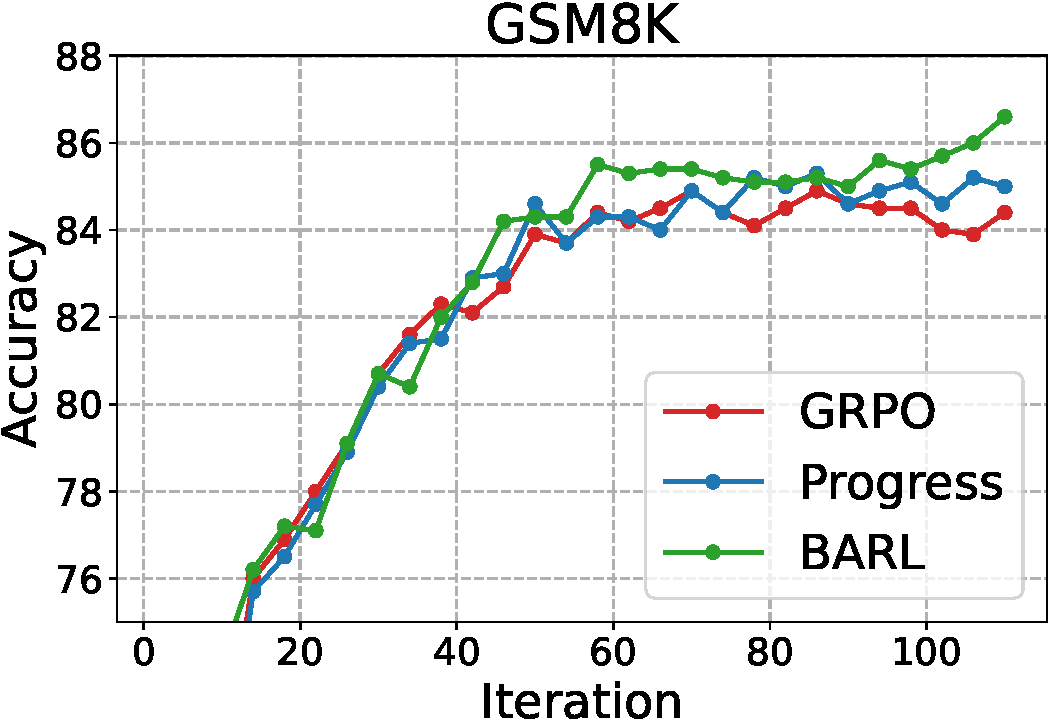
\includegraphics[width=\linewidth]{figs/15b_figs/qwen15_gsm.pdf}
    \end{minipage}
    \begin{minipage}[b]{0.32\linewidth}
        \centering
        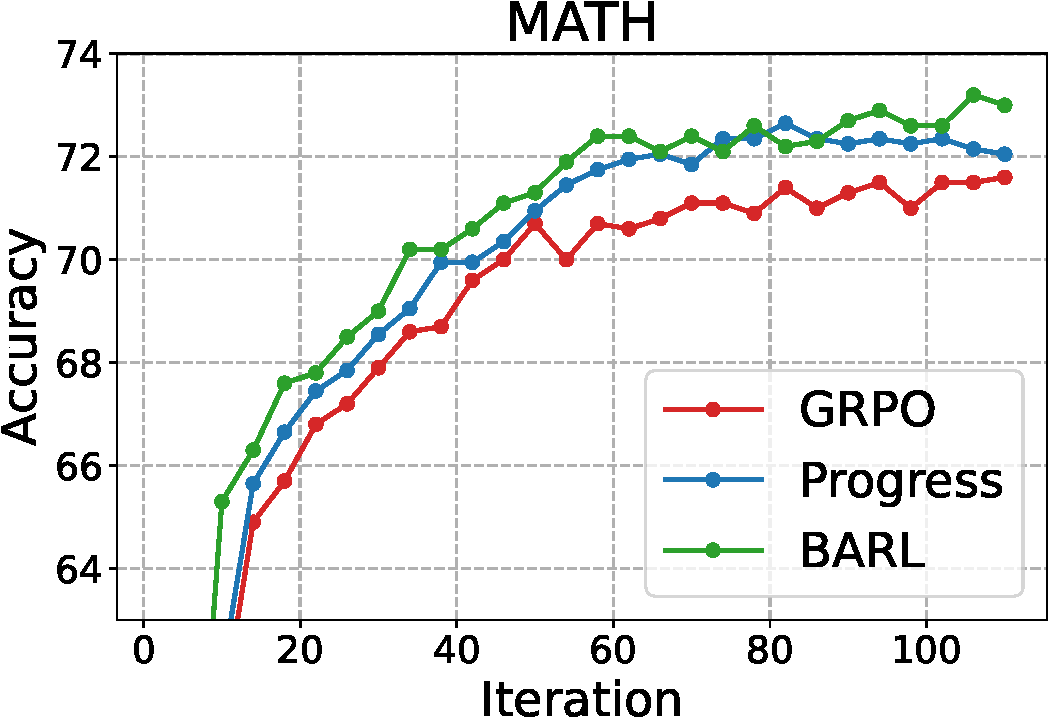
\includegraphics[width=\linewidth]{figs/15b_figs/qwen15_math.pdf}
    \end{minipage}
    \begin{minipage}[b]{0.32\linewidth}
        \centering
        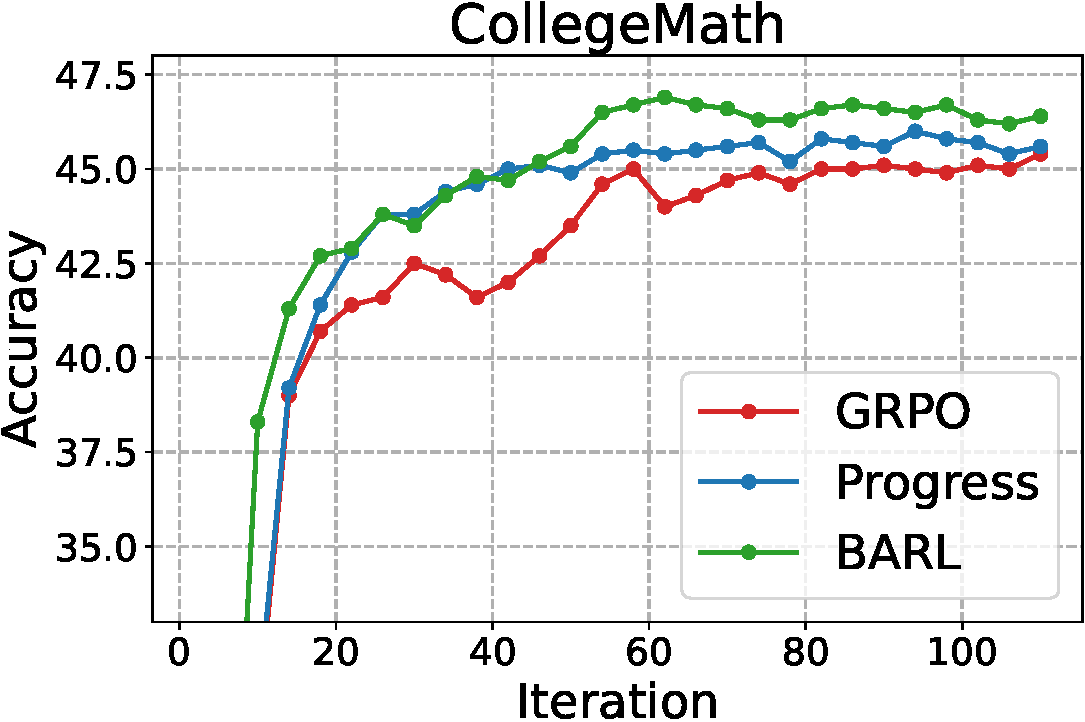
\includegraphics[width=\linewidth]{figs/15b_figs/qwen15_collegemath.pdf}
    \end{minipage}\\
        \begin{minipage}[b]{0.32\linewidth}
        \centering
    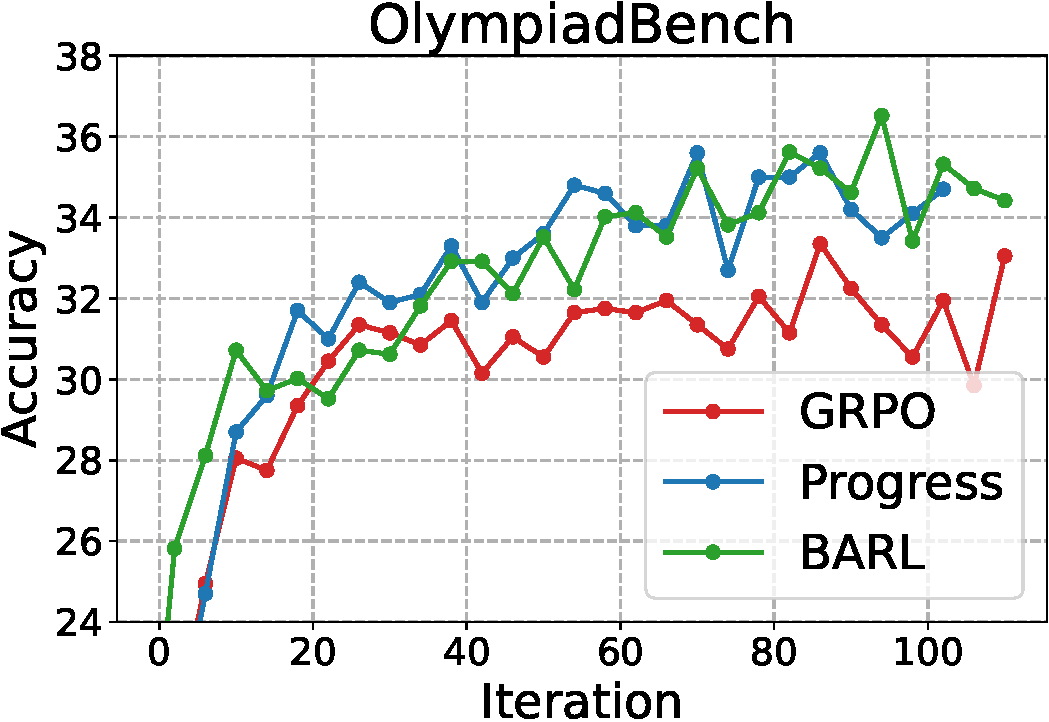
\includegraphics[width=\linewidth]{figs/15b_figs/qwen15_olympiad.pdf}
    \end{minipage}
    \begin{minipage}[b]{0.32\linewidth}
        \centering
    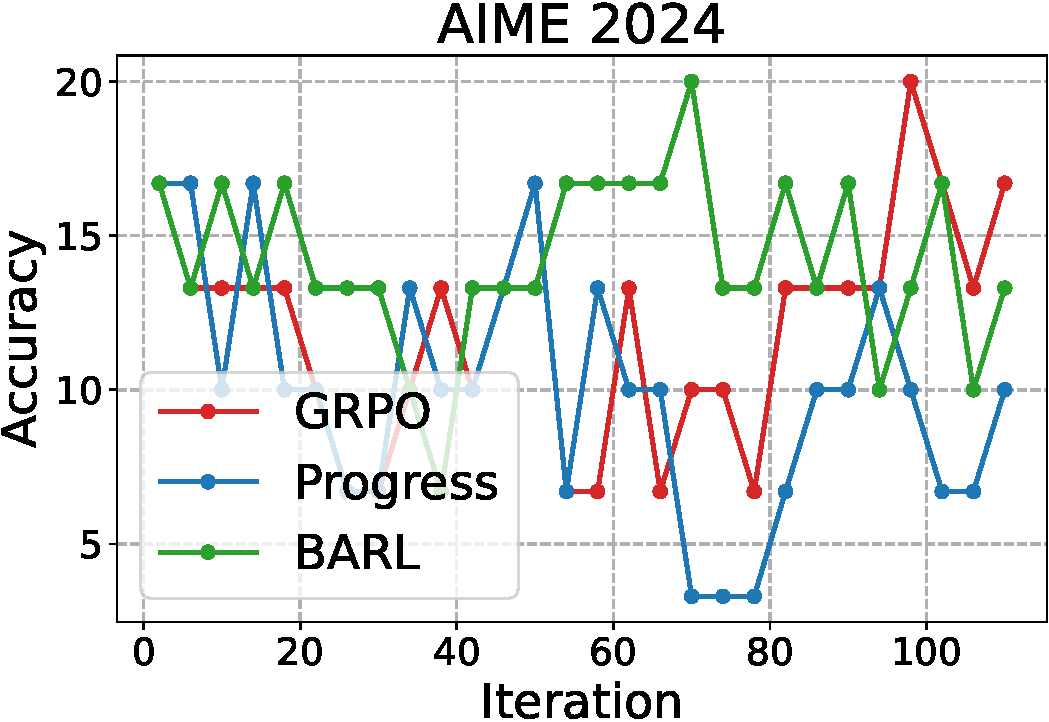
\includegraphics[width=\linewidth]{figs/15b_figs/qwen15_aime.pdf}
    \end{minipage}
    \begin{minipage}[b]{0.32\linewidth}
        \centering
    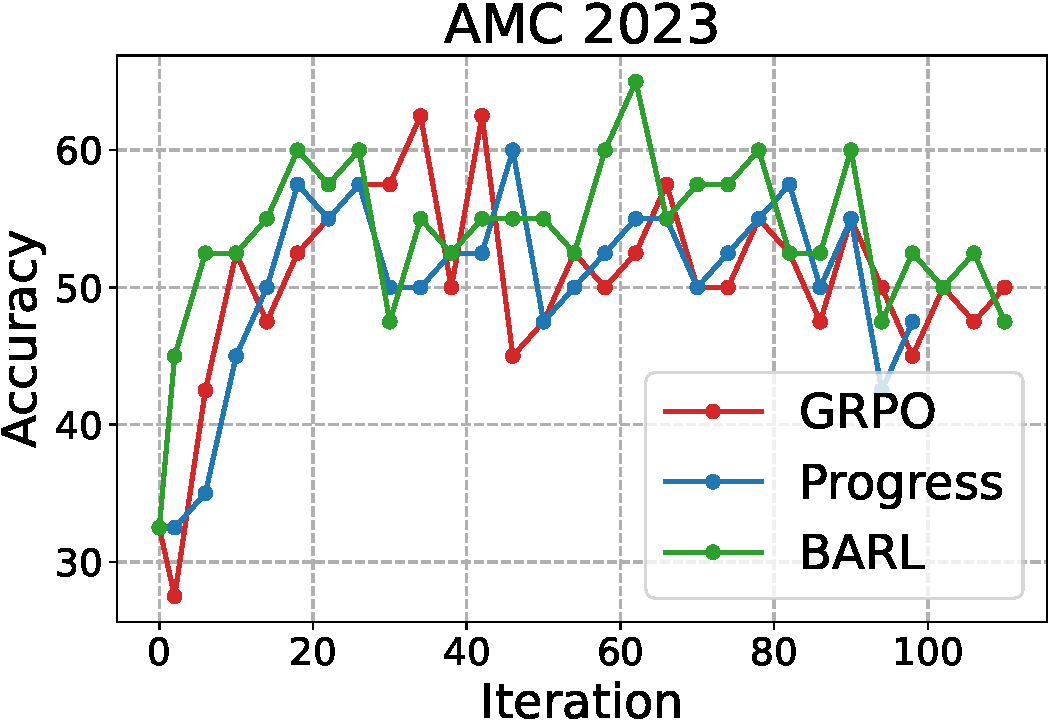
\includegraphics[width=\linewidth]{figs/15b_figs/qwen15_amc.pdf}
    \end{minipage}
\vspace{-0.25cm}
\setlength{\belowcaptionskip}{-15pt}
\caption{Average evaluation accuracies over training iterations for Qwen2.5-Math-1.5B models.}
\label{app_15_acc}
\end{figure}


\begin{figure}[h]
    \centering
    \begin{minipage}[b]{0.32\linewidth}
        \centering
        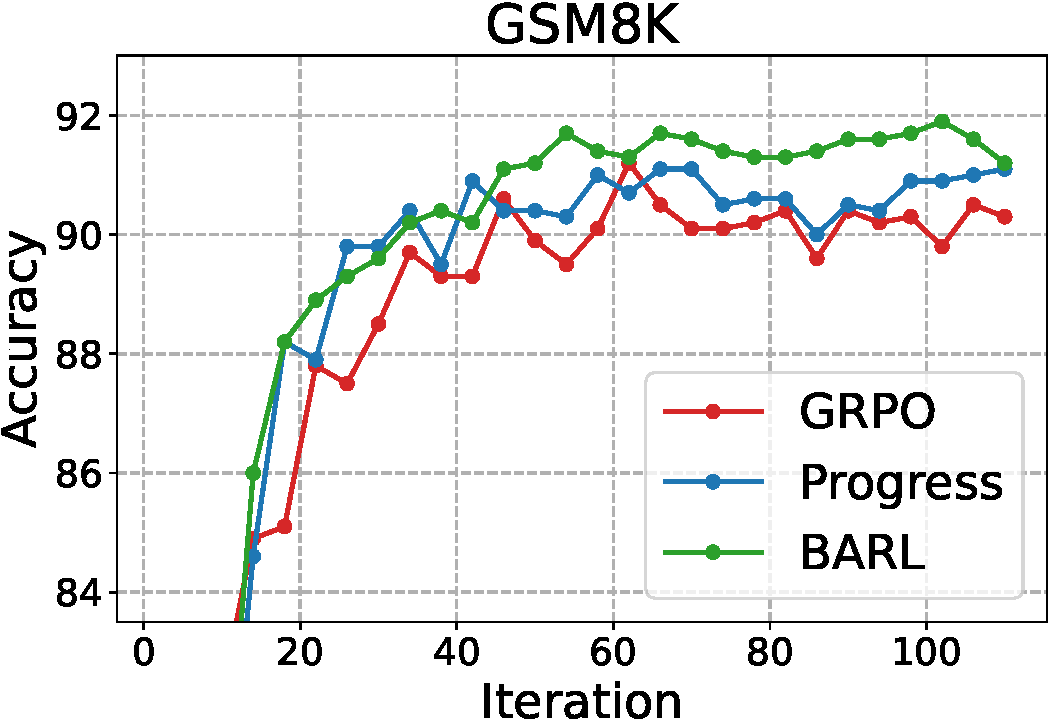
\includegraphics[width=\linewidth]{figs/7b_figs/qwen7_gsm.pdf}
    \end{minipage}
    \begin{minipage}[b]{0.32\linewidth}
        \centering
        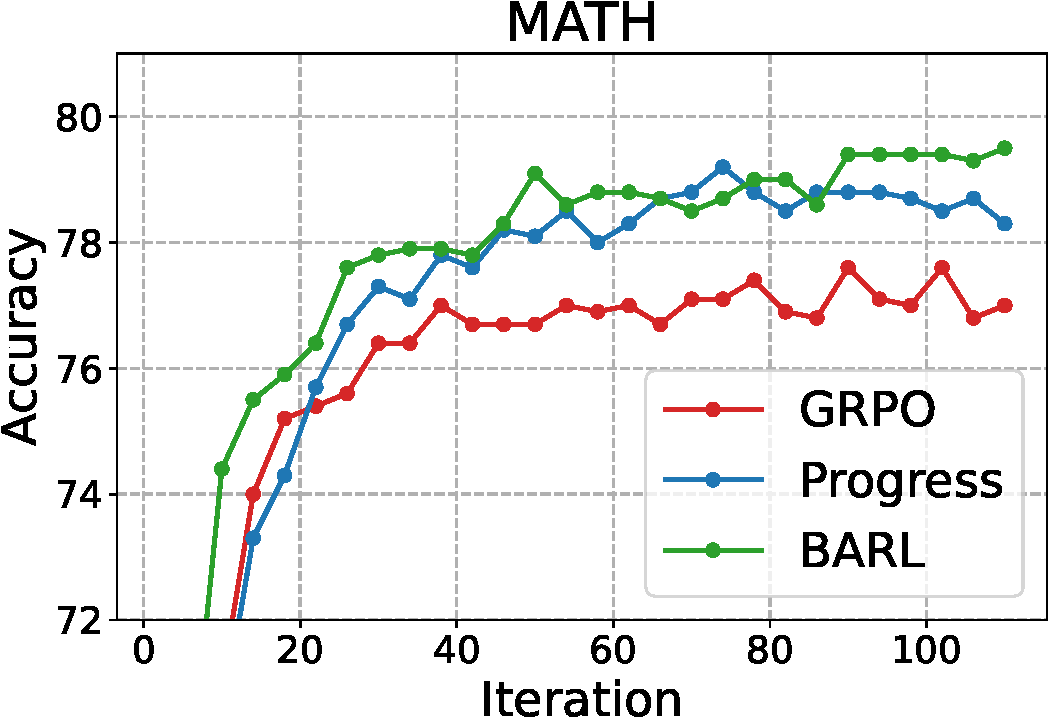
\includegraphics[width=\linewidth]{figs/7b_figs/qwen7_MATH.pdf}
    \end{minipage}
    \begin{minipage}[b]{0.32\linewidth}
        \centering
        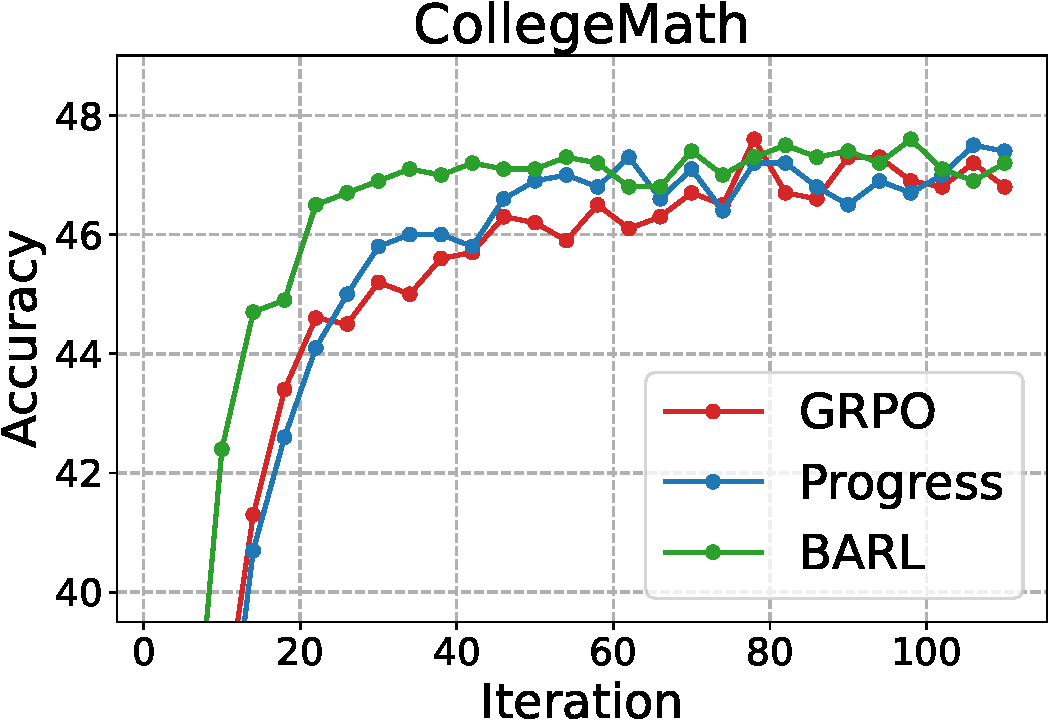
\includegraphics[width=\linewidth]{figs/7b_figs/qwen7_CollegeMath.pdf}
    \end{minipage}\\
        \begin{minipage}[b]{0.32\linewidth}
        \centering
    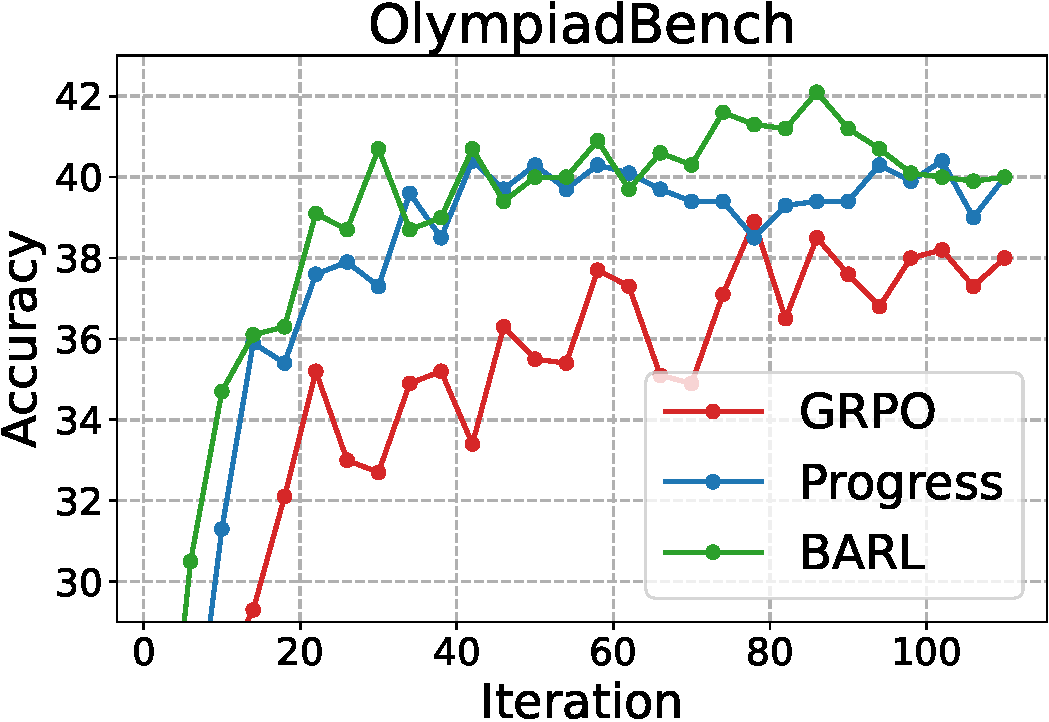
\includegraphics[width=\linewidth]{figs/7b_figs/qwen7_olympiad.pdf}
    \end{minipage}
    \begin{minipage}[b]{0.32\linewidth}
        \centering
    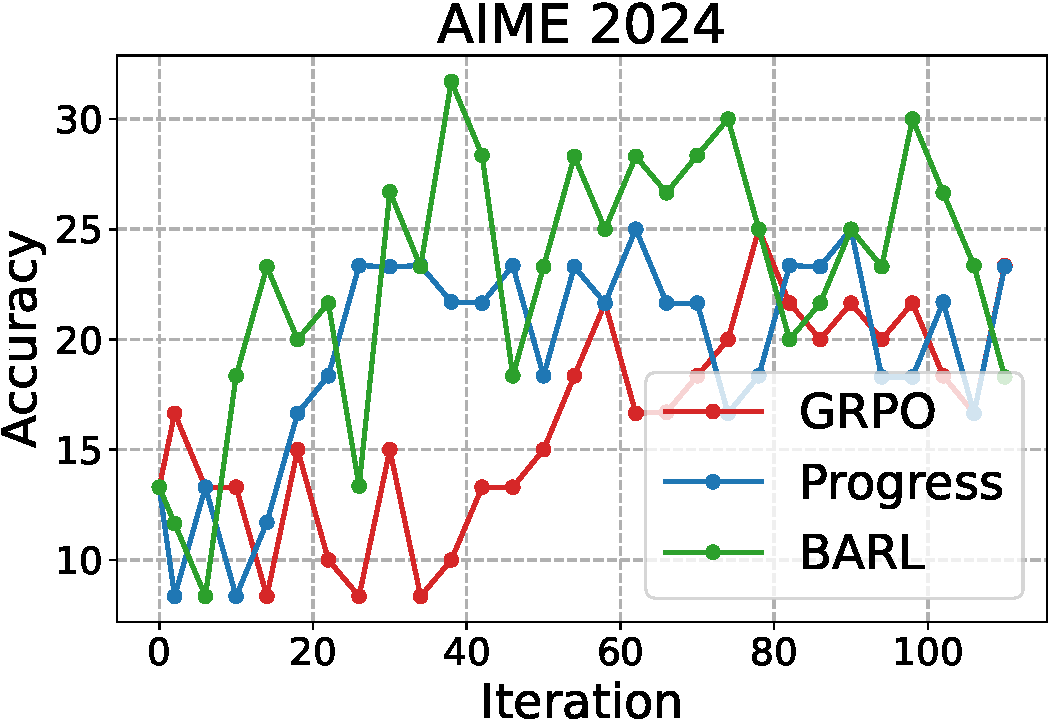
\includegraphics[width=\linewidth]{figs/7b_figs/qwen7_aime.pdf}
    \end{minipage}
    \begin{minipage}[b]{0.32\linewidth}
        \centering
    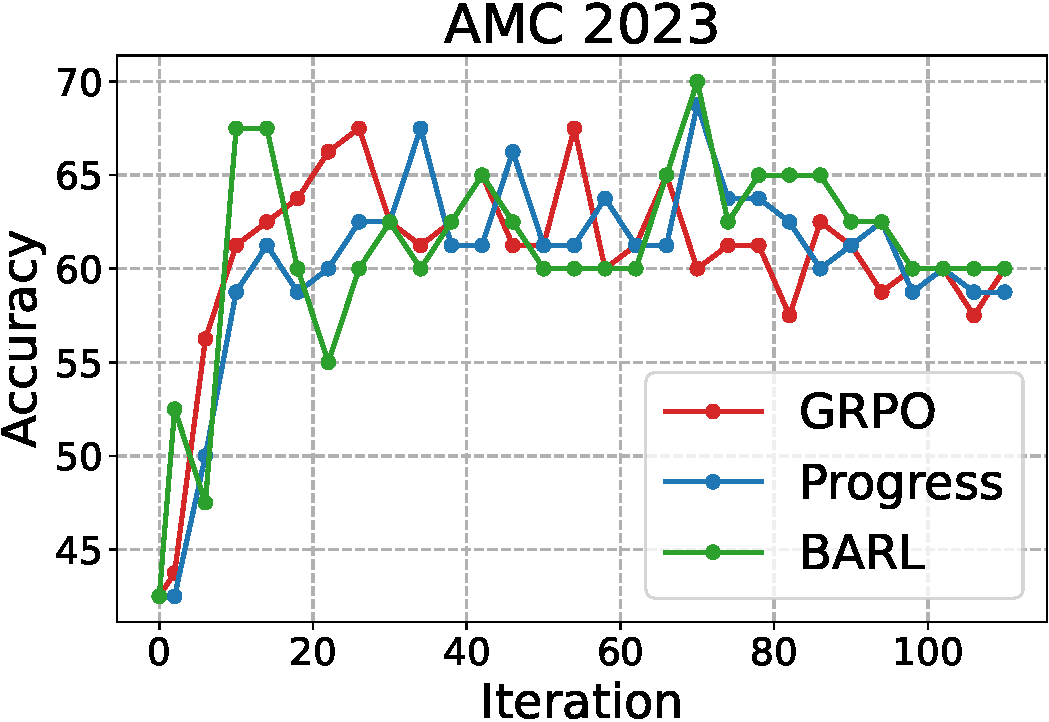
\includegraphics[width=\linewidth]{figs/7b_figs/qwen7_amc.pdf}
    \end{minipage}
\vspace{-0.25cm}
\setlength{\belowcaptionskip}{-15pt}
\caption{Average evaluation accuracies over training iterations for Qwen2.5-Math-7B models.}
\label{app_7_acc}
\end{figure}

\begin{figure}[h]
    \centering
    \begin{minipage}[b]{0.32\linewidth}
        \centering
        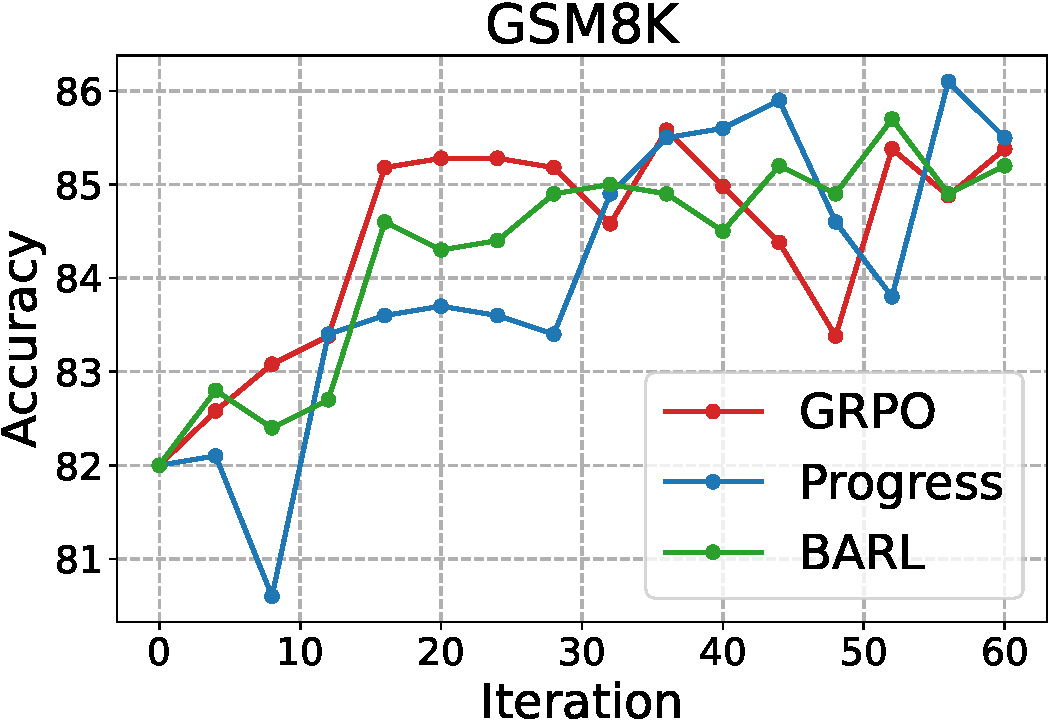
\includegraphics[width=\linewidth]{figs/8b_figs/dsllama_gsm.pdf}
    \end{minipage}
    \begin{minipage}[b]{0.32\linewidth}
        \centering
        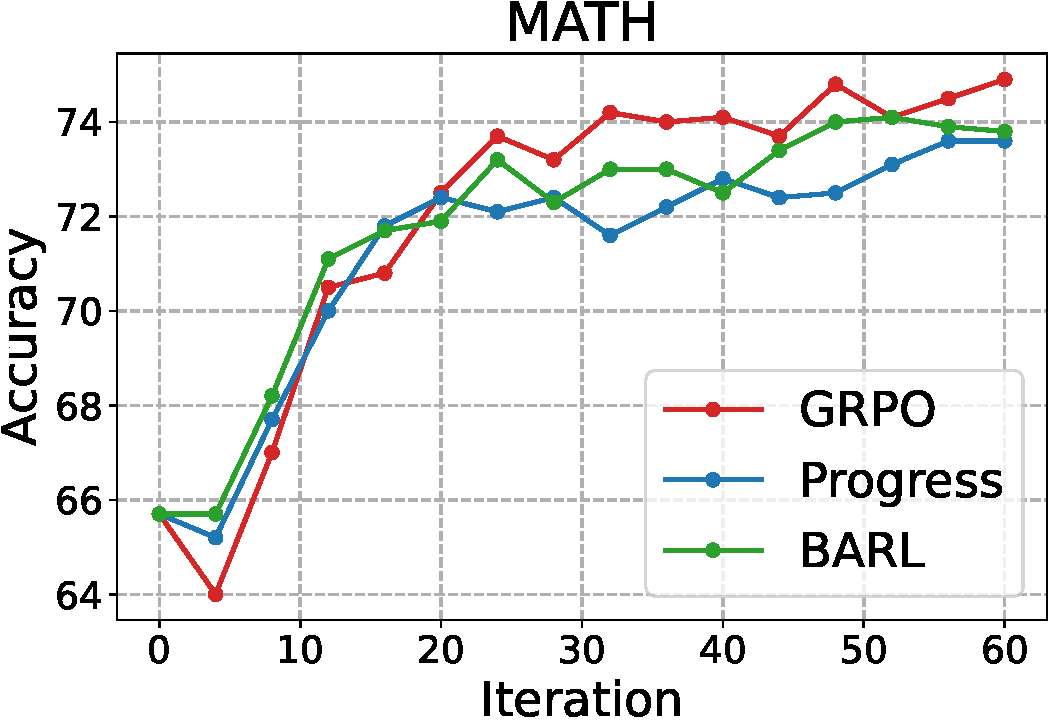
\includegraphics[width=\linewidth]{figs/8b_figs/dsllama_math.pdf}
    \end{minipage}
    \begin{minipage}[b]{0.32\linewidth}
        \centering
        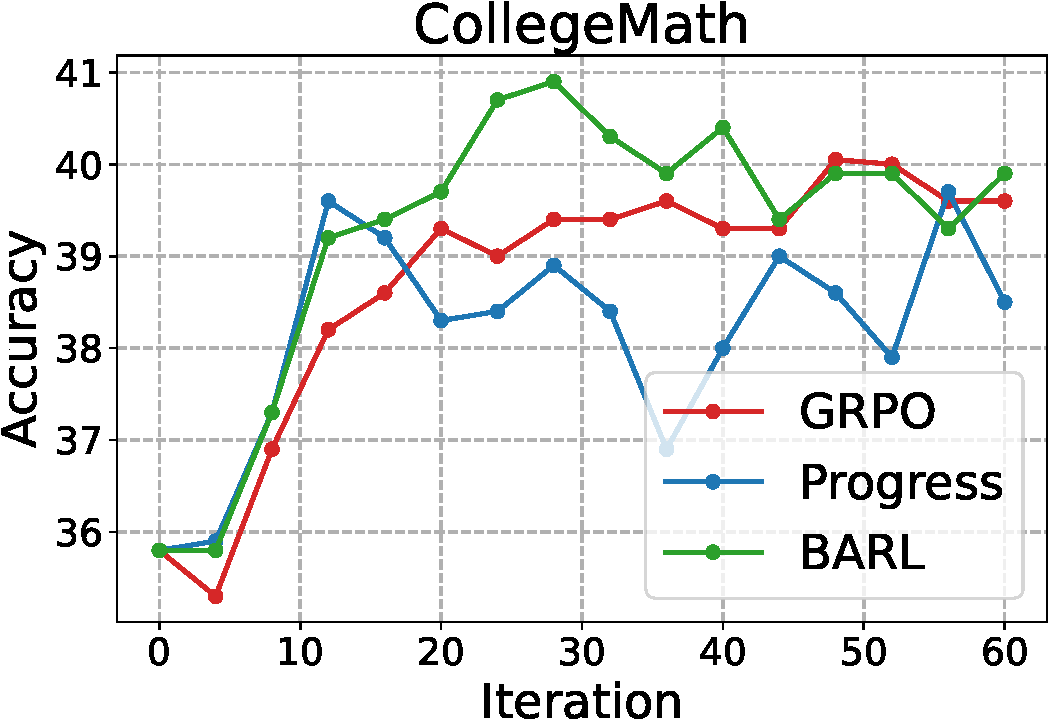
\includegraphics[width=\linewidth]{figs/8b_figs/dsllama_collegemath.pdf}
    \end{minipage}\\
        \begin{minipage}[b]{0.32\linewidth}
        \centering
    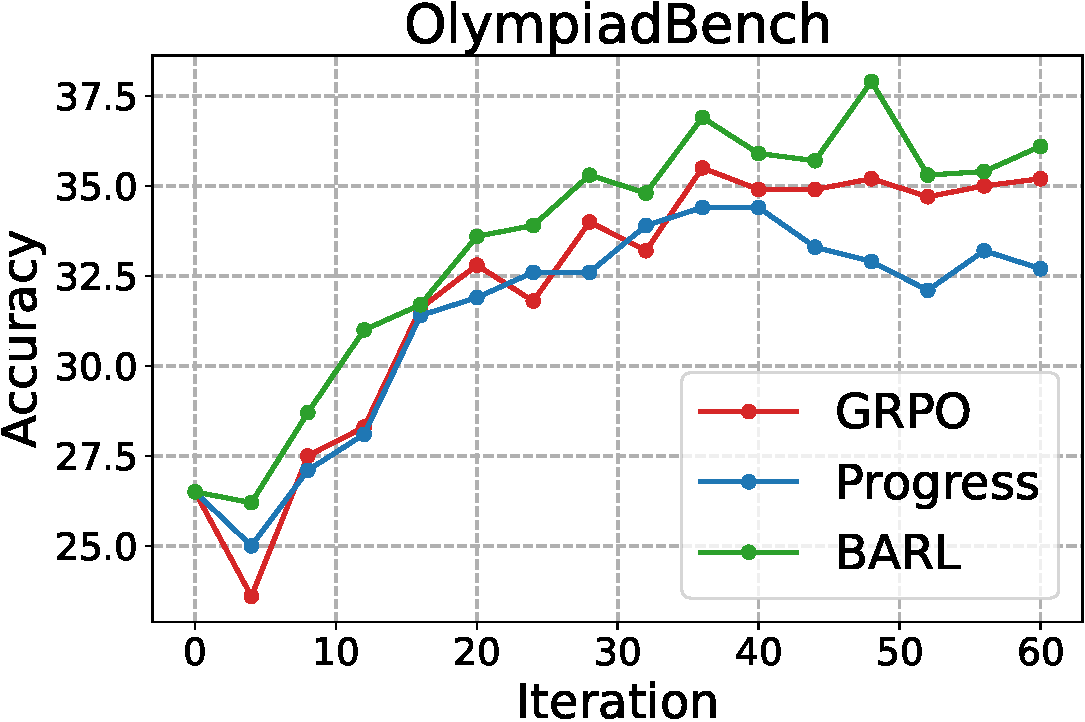
\includegraphics[width=\linewidth]{figs/8b_figs/dsllama_olym.pdf}
    \end{minipage}
    \begin{minipage}[b]{0.32\linewidth}
        \centering
    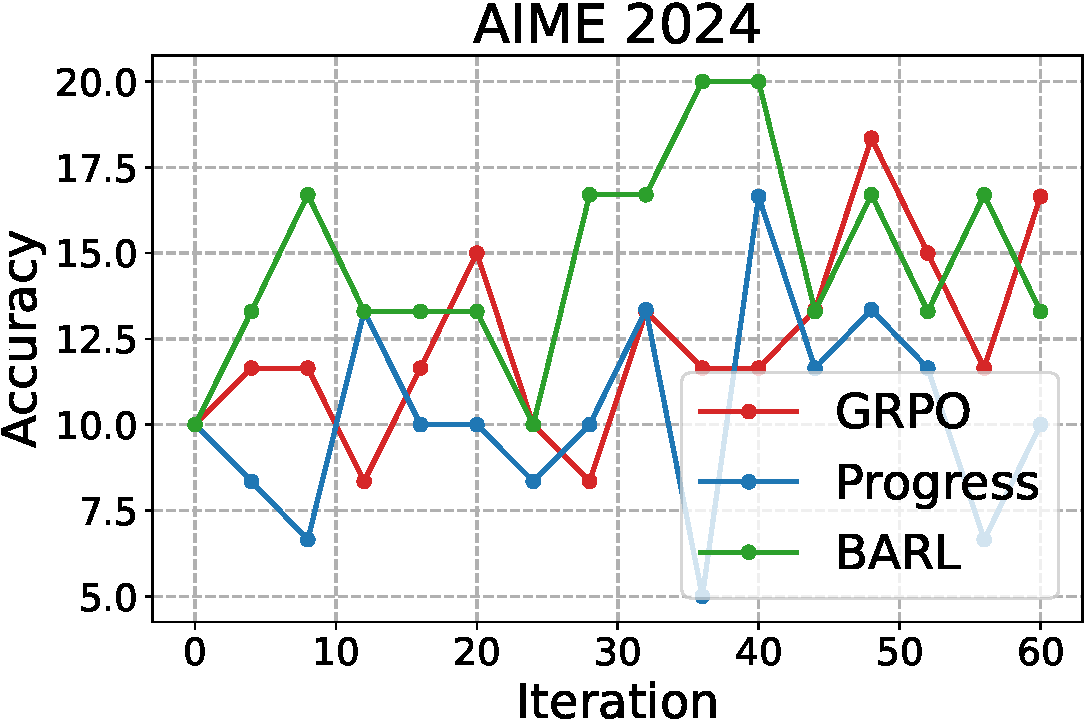
\includegraphics[width=\linewidth]{figs/8b_figs/dsllama_aime.pdf}
    \end{minipage}
    \begin{minipage}[b]{0.32\linewidth}
        \centering
    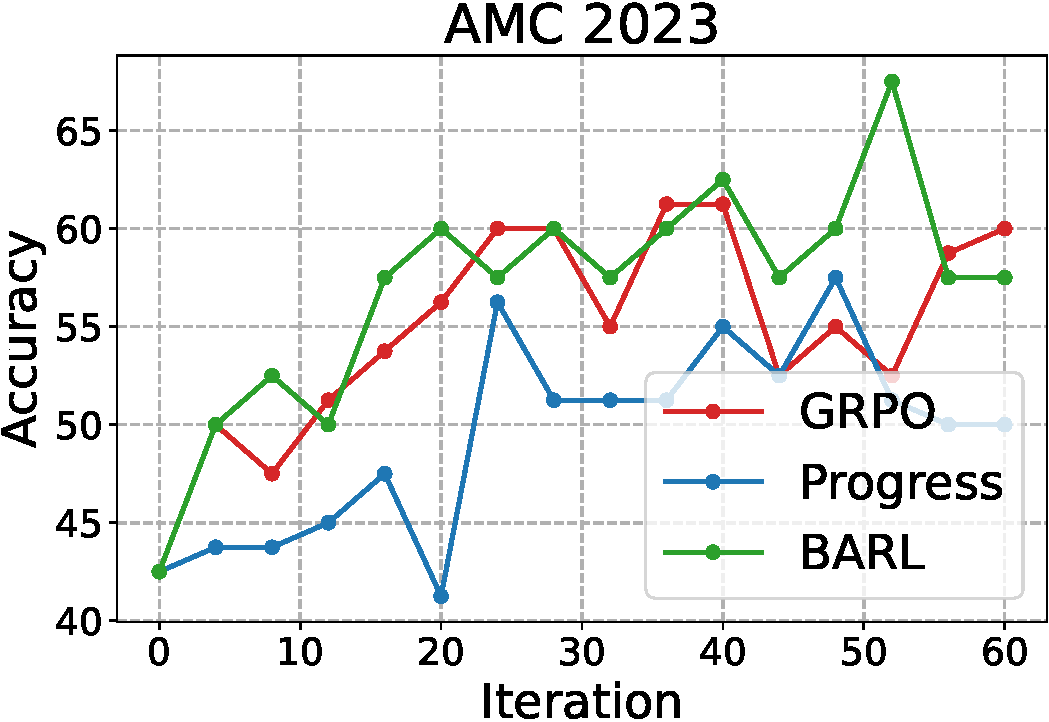
\includegraphics[width=\linewidth]{figs/8b_figs/dsllama_amc.pdf}
    \end{minipage}
\vspace{-0.25cm}
\setlength{\belowcaptionskip}{-10pt}
\caption{Average evaluation accuracies over training iterations for R1-Distill-Llama-8B models.}
\label{app_8_acc}
\end{figure}

\newpage
\subsection{Evaluation Results: Response Lengths}\label{app_len_eval}
In this section, we present the evolution of evaluation response lengths over training iterations for Qwen2.5-Math-1.5B, Qwen2.5-Math-7B, and DeepSeek-R1-Distill-Llama-8B, shown in Figures \ref{app_15_len}, \ref{app_7_len}, and \ref{app_8_len}, respectively. Across most benchmarks, response lengths tend to decrease as training progresses for all algorithms. The response length during training has a very similar trend to that during evaluation. This trend arises because all three models exhibit reflective behaviors, such as self-evaluation and backtracking, that introduce redundant tokens and lengthen responses. As shown in Figure \ref{fig_ablation_value}, these behaviors are likely superficial or stylistic patterns with limited effectiveness. An exception is AIME, where some models maintain consistently long responses due to the benchmark’s intrinsic requirement for extended reasoning, even under optimal non-reflective policies.
\begin{figure}[h]
    \centering
    \begin{minipage}[b]{0.32\linewidth}
        \centering
        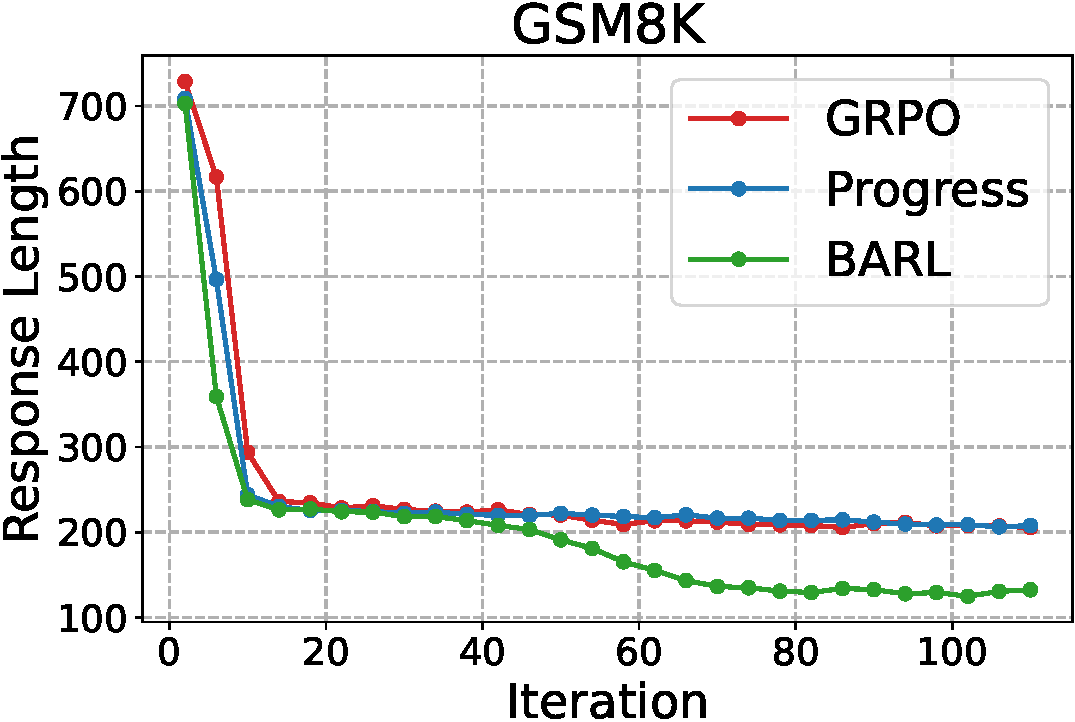
\includegraphics[width=\linewidth]{figs/15b_figs/qwen15_gsm_len.pdf}
    \end{minipage}
    \begin{minipage}[b]{0.32\linewidth}
        \centering
        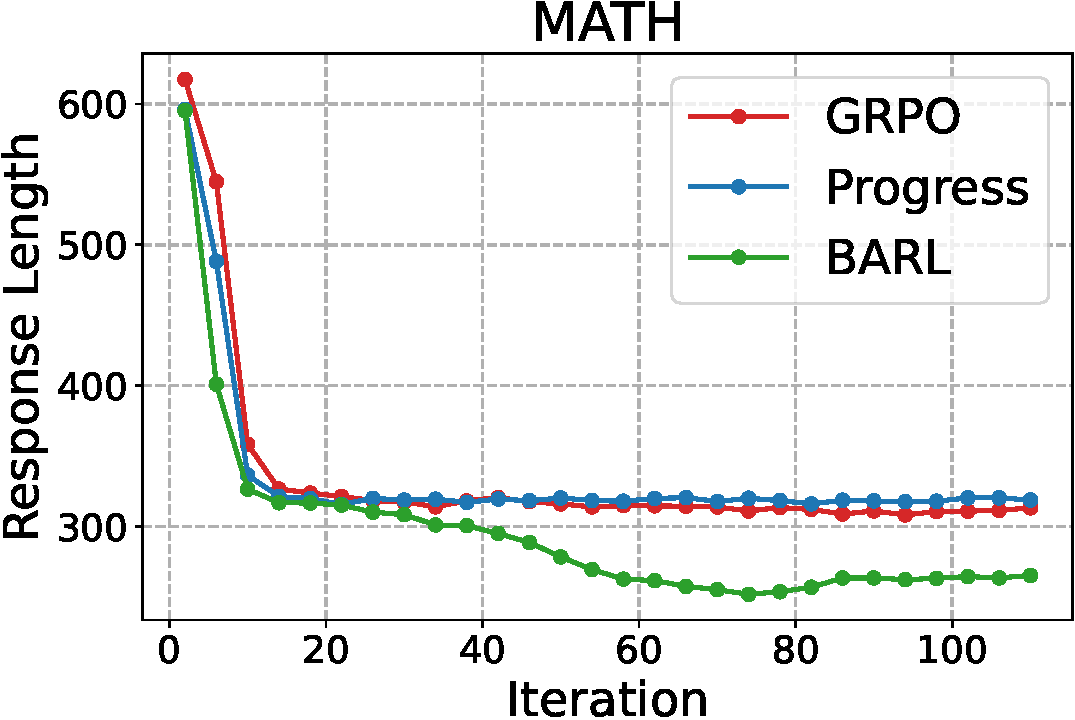
\includegraphics[width=\linewidth]{figs/15b_figs/qwen15_math_len.pdf}
    \end{minipage}
    \begin{minipage}[b]{0.32\linewidth}
        \centering
        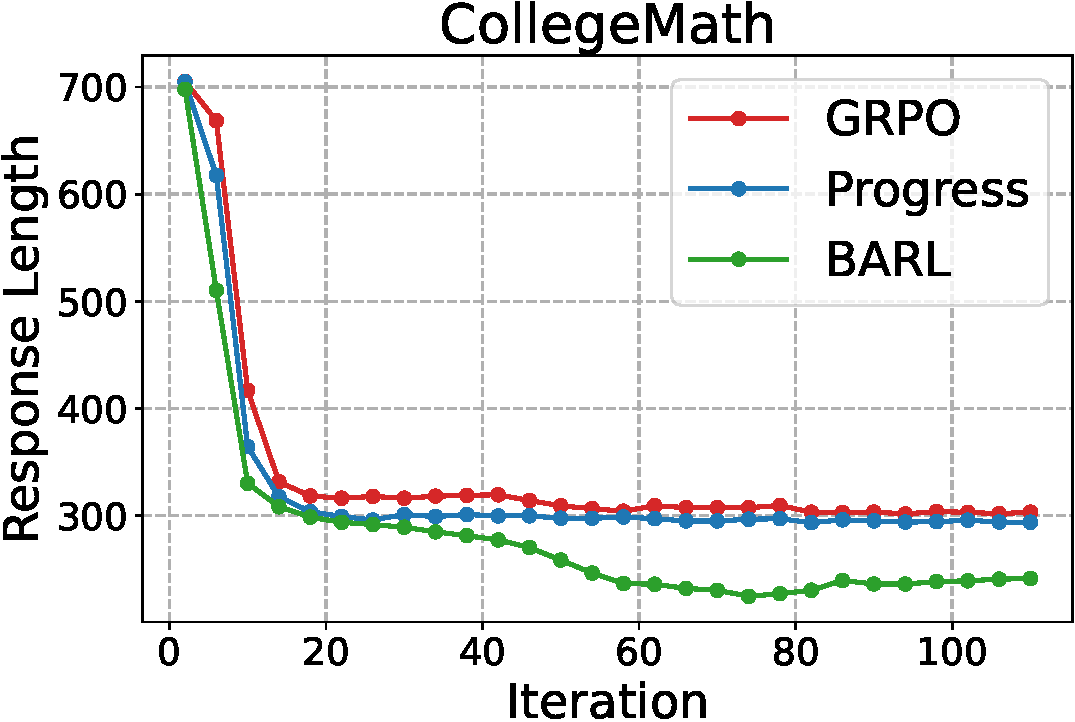
\includegraphics[width=\linewidth]{figs/15b_figs/qwen15_collegemath_len.pdf}
    \end{minipage}\\
        \begin{minipage}[b]{0.32\linewidth}
        \centering
    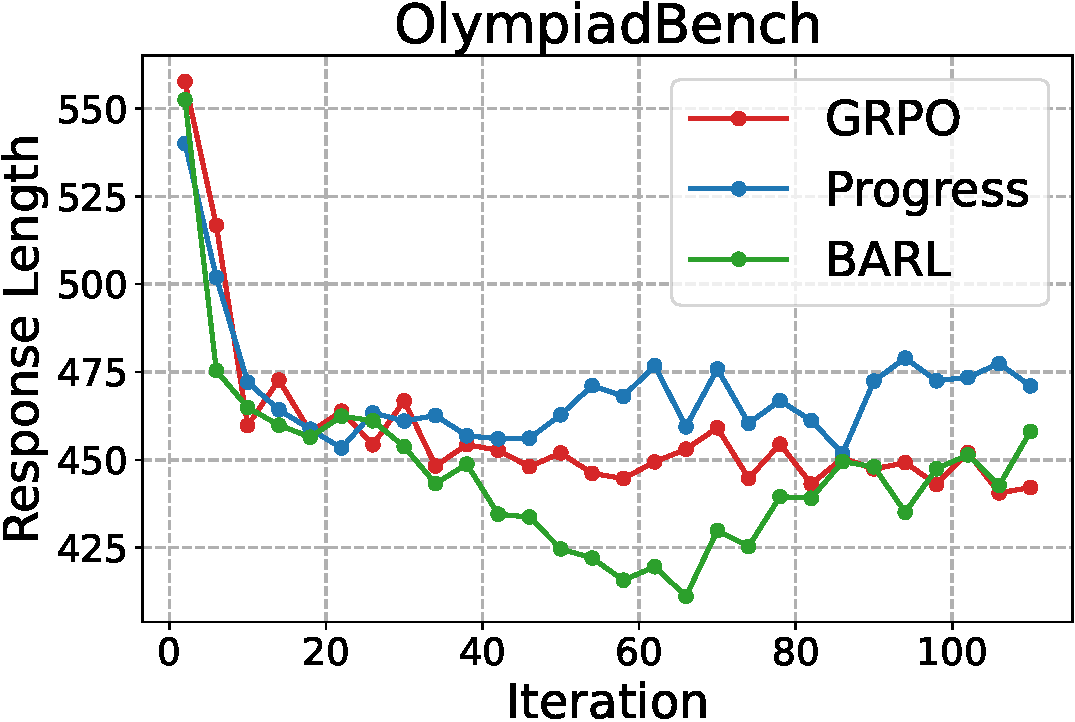
\includegraphics[width=\linewidth]{figs/15b_figs/qwen15_olym_len.pdf}
    \end{minipage}
    \begin{minipage}[b]{0.32\linewidth}
        \centering
    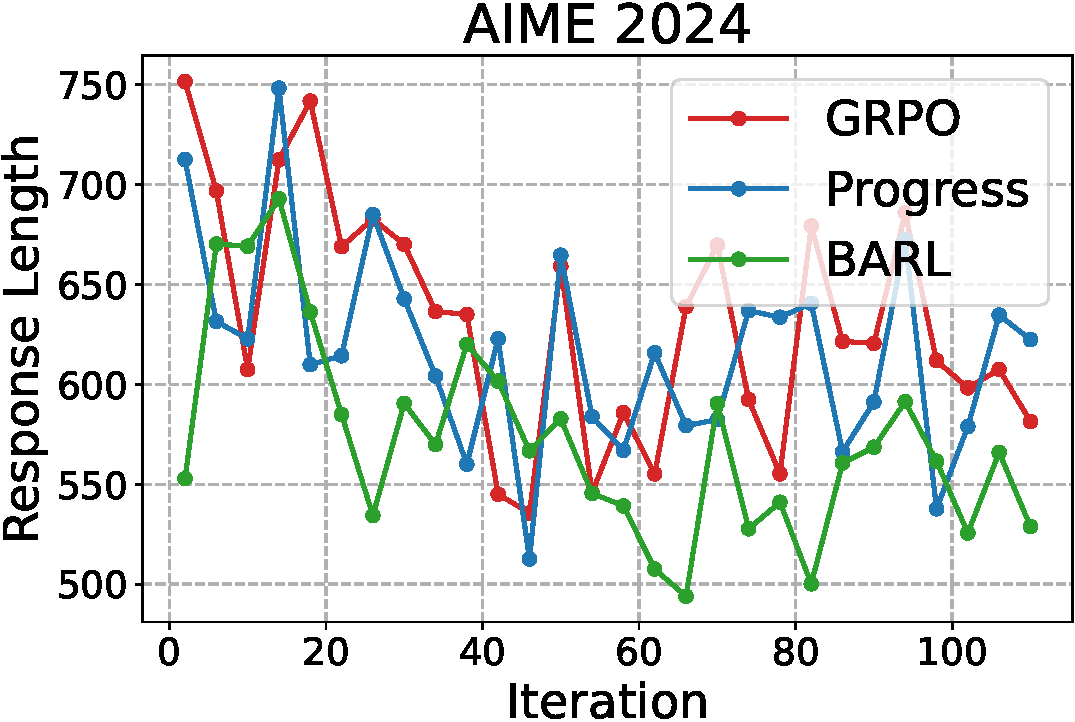
\includegraphics[width=\linewidth]{figs/15b_figs/qwen15_aime_len.pdf}
    \end{minipage}
    \begin{minipage}[b]{0.32\linewidth}
        \centering
    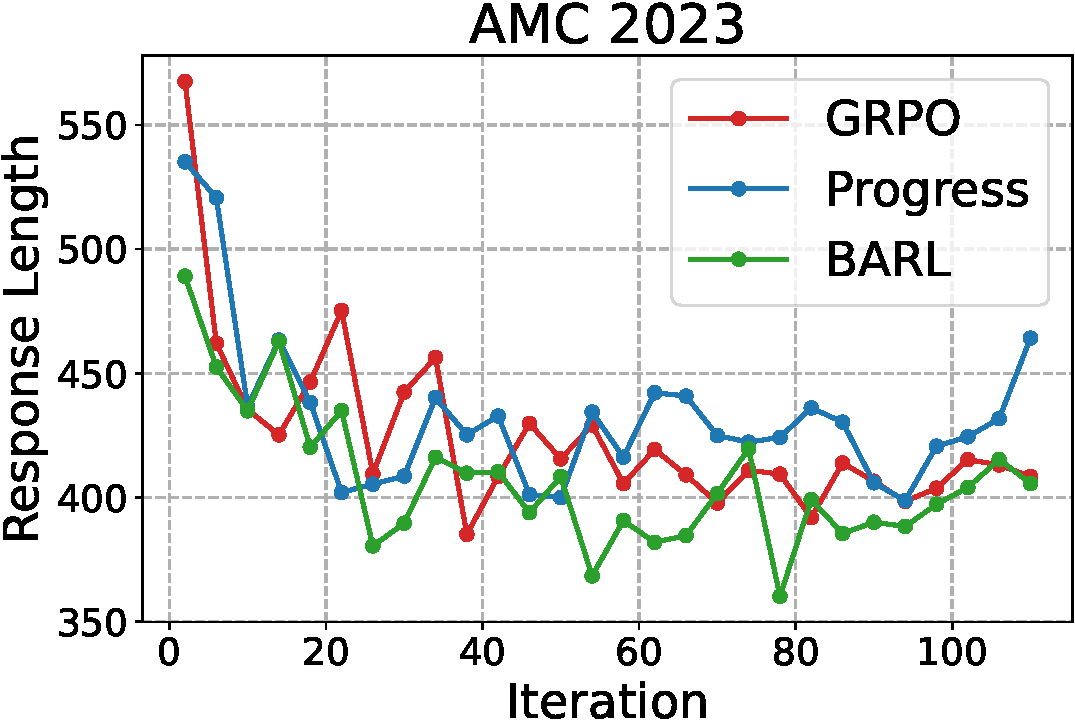
\includegraphics[width=\linewidth]{figs/15b_figs/qwen15_amc_len.pdf}
    \end{minipage}
\vspace{-0.1cm}
\setlength{\belowcaptionskip}{-10pt}
\caption{Average evaluation response lengths over training iterations for Qwen2.5-Math-1.5B models.}
\label{app_15_len}
\end{figure}

\begin{figure}[h]
    \centering
    \begin{minipage}[b]{0.32\linewidth}
        \centering
        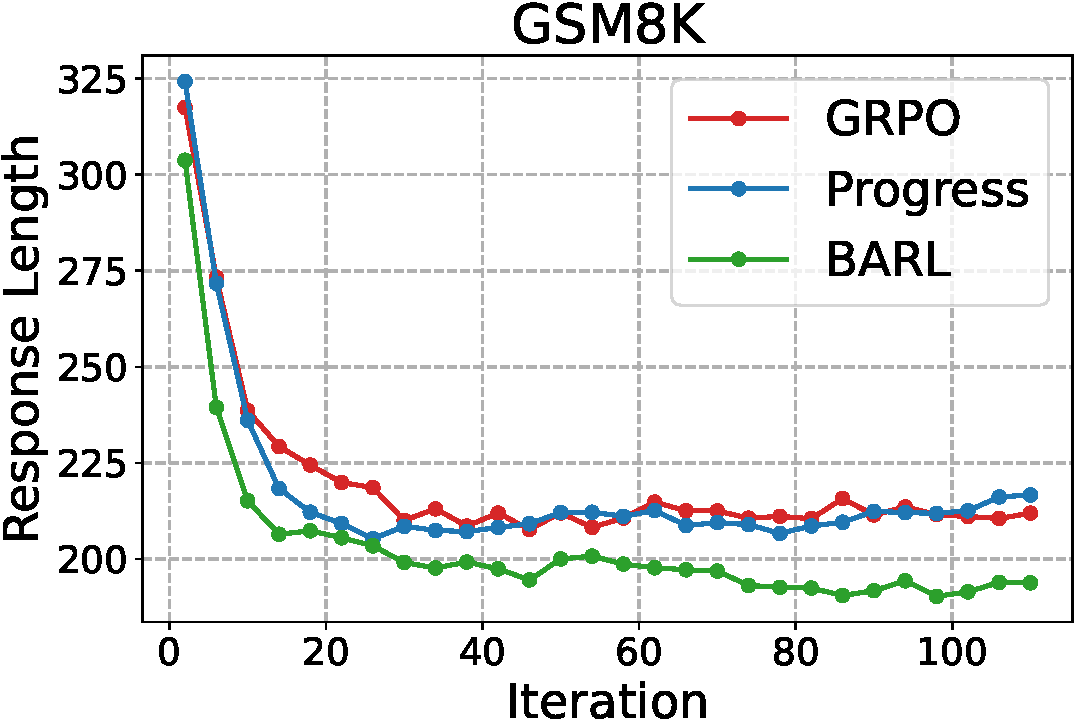
\includegraphics[width=\linewidth]{figs/7b_figs/qwen7_gsm_len.pdf}
    \end{minipage}
    \begin{minipage}[b]{0.32\linewidth}
        \centering
        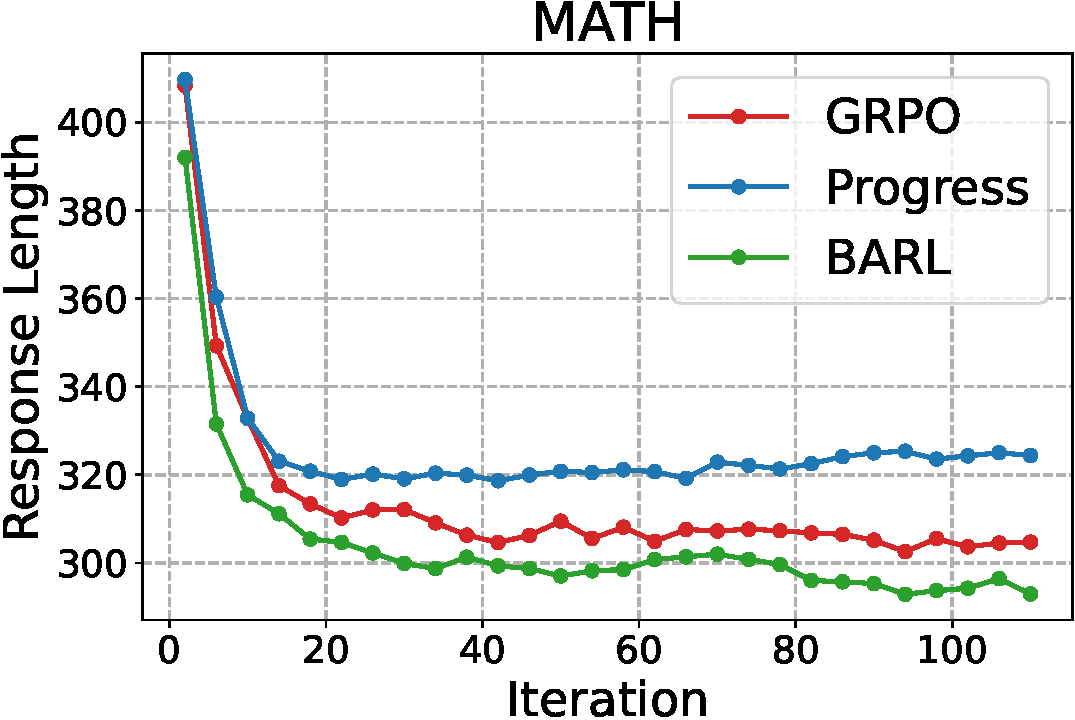
\includegraphics[width=\linewidth]{figs/7b_figs/qwen7_math_len.pdf}
    \end{minipage}
    \begin{minipage}[b]{0.32\linewidth}
        \centering
        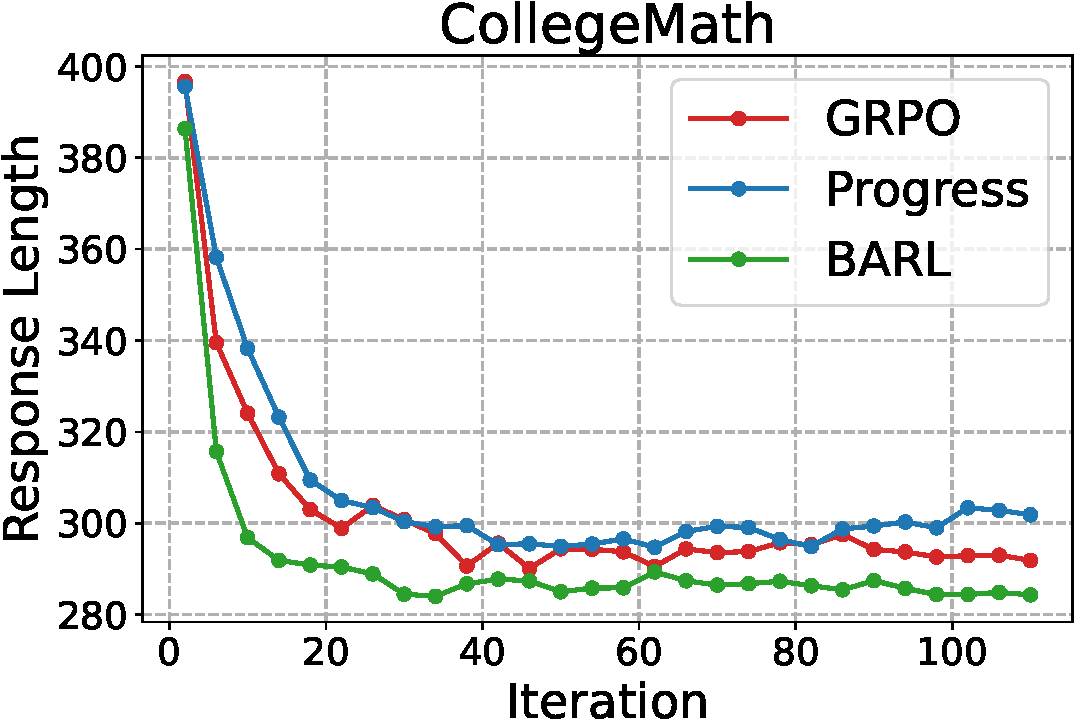
\includegraphics[width=\linewidth]{figs/7b_figs/qwen7_collegemath_len.pdf}
    \end{minipage}\\
        \begin{minipage}[b]{0.32\linewidth}
        \centering
    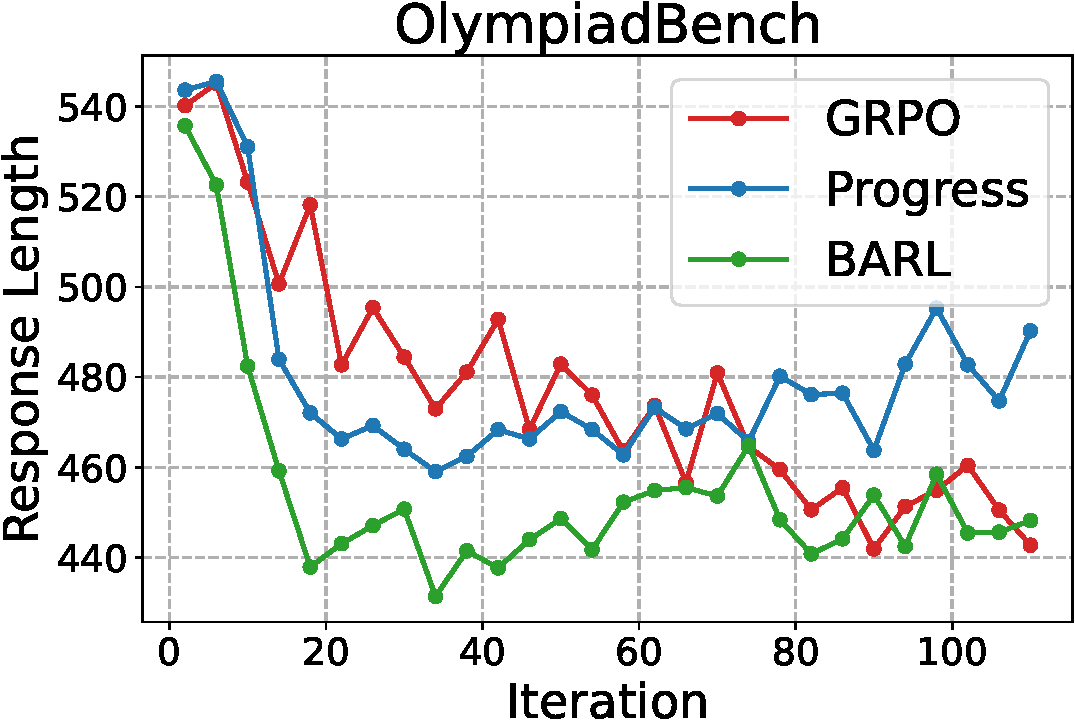
\includegraphics[width=\linewidth]{figs/7b_figs/qwen7_olym_len.pdf}
    \end{minipage}
    \begin{minipage}[b]{0.32\linewidth}
        \centering
    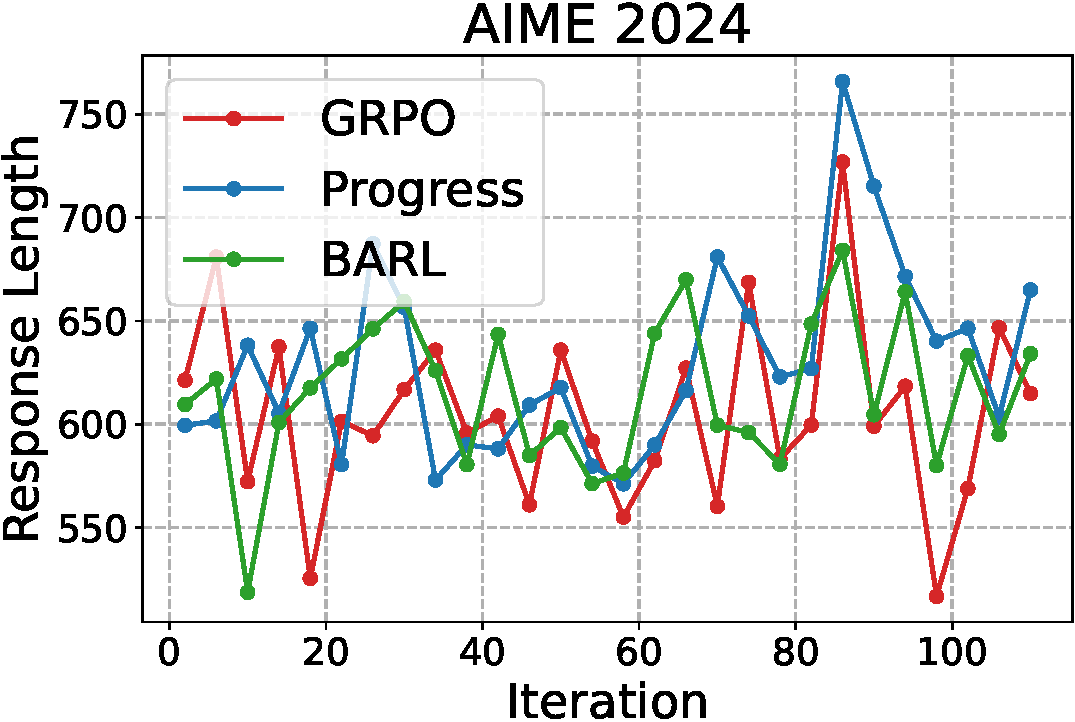
\includegraphics[width=\linewidth]{figs/7b_figs/qwen7_aime_len.pdf}
    \end{minipage}
    \begin{minipage}[b]{0.32\linewidth}
        \centering
    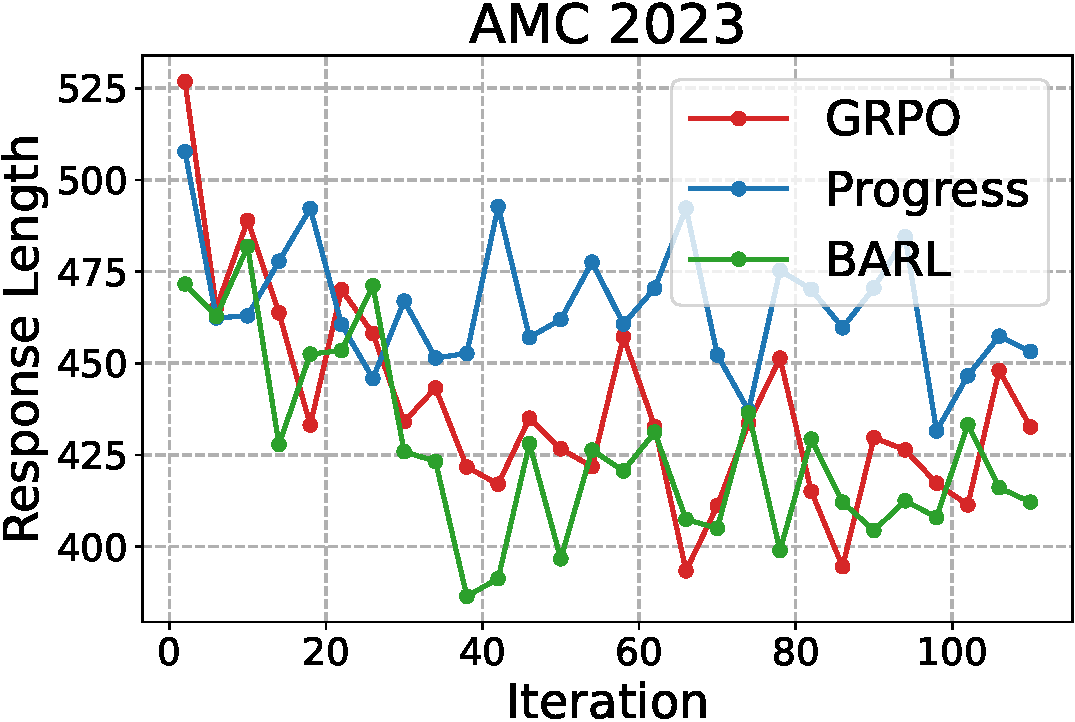
\includegraphics[width=\linewidth]{figs/7b_figs/qwen7_amc_len.pdf}
    \end{minipage}
\vspace{-0.1cm}
\setlength{\belowcaptionskip}{-10pt}
\caption{Average evaluation response lengths over training iterations for Qwen2.5-Math-7B models.}
\label{app_7_len}
\end{figure}


\begin{figure}[h]
    \centering
    \begin{minipage}[b]{0.32\linewidth}
        \centering
        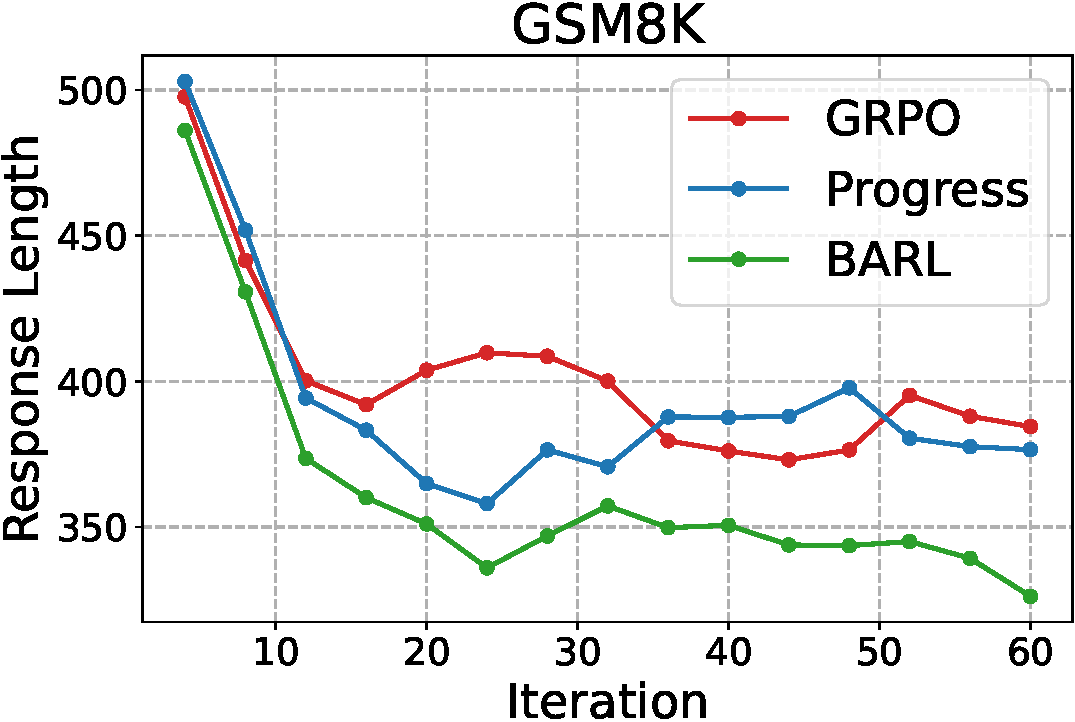
\includegraphics[width=\linewidth]{figs/8b_figs/dsllama_gsm_len.pdf}
    \end{minipage}
    \begin{minipage}[b]{0.32\linewidth}
        \centering
        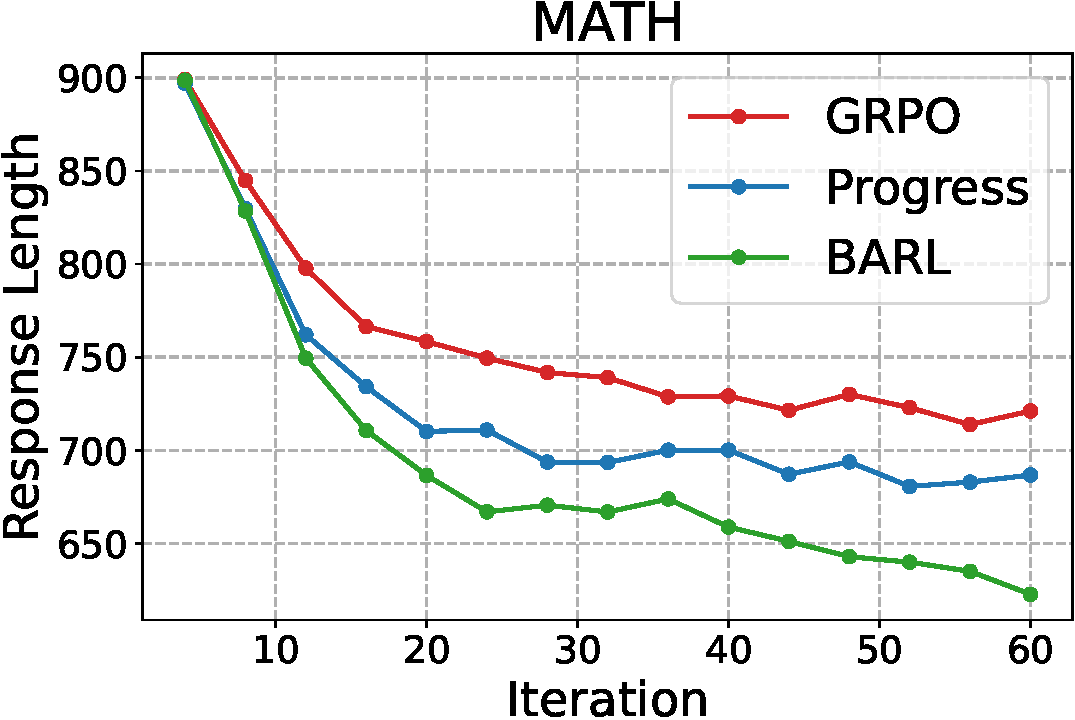
\includegraphics[width=\linewidth]{figs/8b_figs/dsllama_math_len.pdf}
    \end{minipage}
    \begin{minipage}[b]{0.32\linewidth}
        \centering
        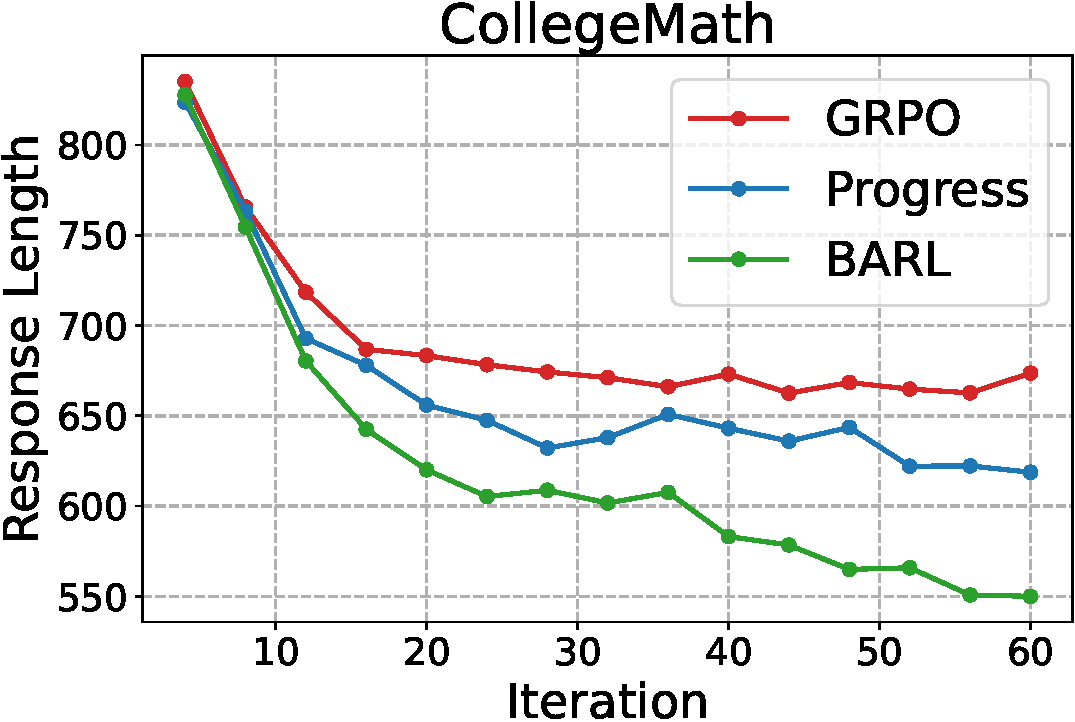
\includegraphics[width=\linewidth]{figs/8b_figs/dsllama_collegemath_len.pdf}
    \end{minipage}\\
        \begin{minipage}[b]{0.32\linewidth}
        \centering
    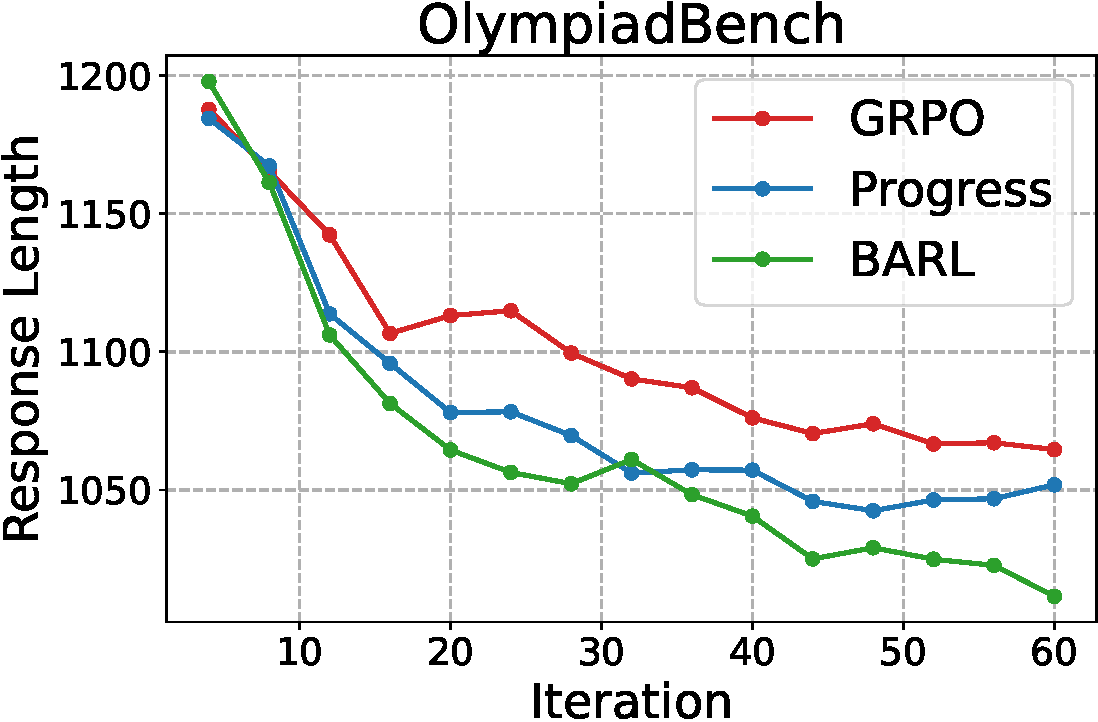
\includegraphics[width=\linewidth]{figs/8b_figs/dsllama_olymp_len.pdf}
    \end{minipage}
    \begin{minipage}[b]{0.32\linewidth}
        \centering
    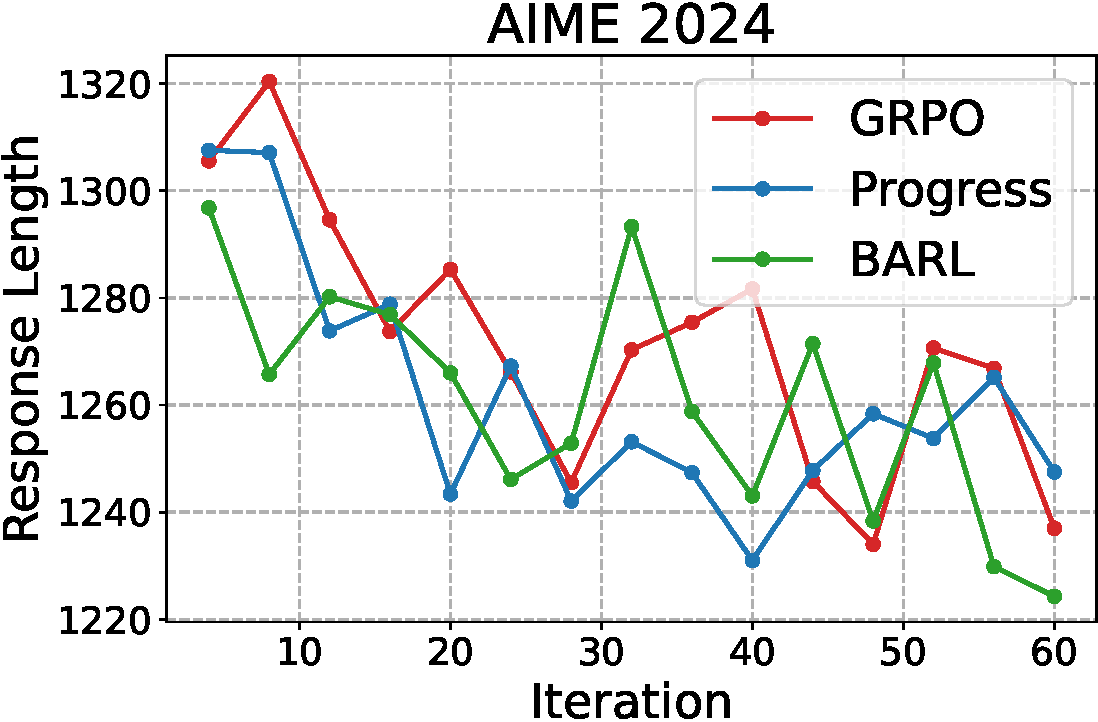
\includegraphics[width=\linewidth]{figs/8b_figs/dsllama_aime_len.pdf}
    \end{minipage}
    \begin{minipage}[b]{0.32\linewidth}
        \centering
    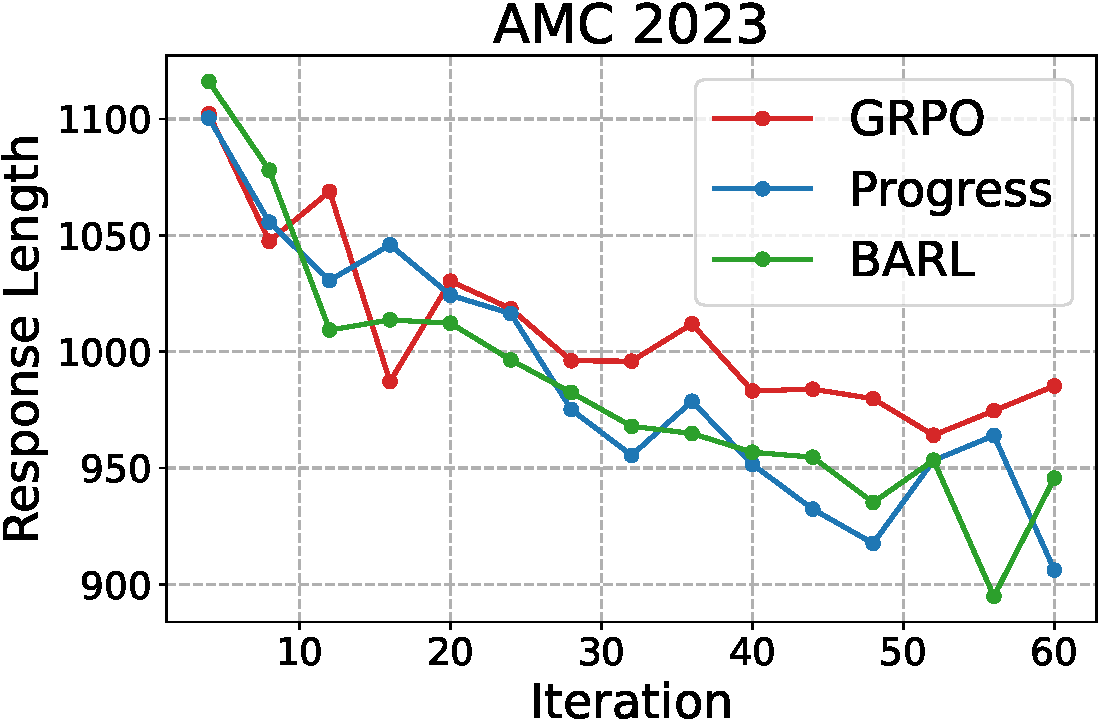
\includegraphics[width=\linewidth]{figs/8b_figs/dsllama_amc_len.pdf}
    \end{minipage}
\vspace{-0.2cm}
\setlength{\belowcaptionskip}{-15pt}
\caption{Average evaluation response lengths over training iterations for R1-Distill-Llama-8B models.}
\label{app_8_len}
\end{figure}

\newpage
Since the models used in the main experiments already exhibit lengthy CoTs with reflective patterns, we further implement BARL on the Llama-3.2-3B-Instruct model, which displays fewer self-reflections. The results are presented in Figure \ref{app_fig_llama3b_res}. Initially, the response length decreases as the base model tends to produce excessively long reasoning traces, often exceeding ten steps, which are pruned during early training. Subsequently, the response length increases, as a result of plausible strategy stitching.

\begin{figure}[htbp]
  \centering
  \begin{minipage}[c]{0.32\textwidth}
    \centering
    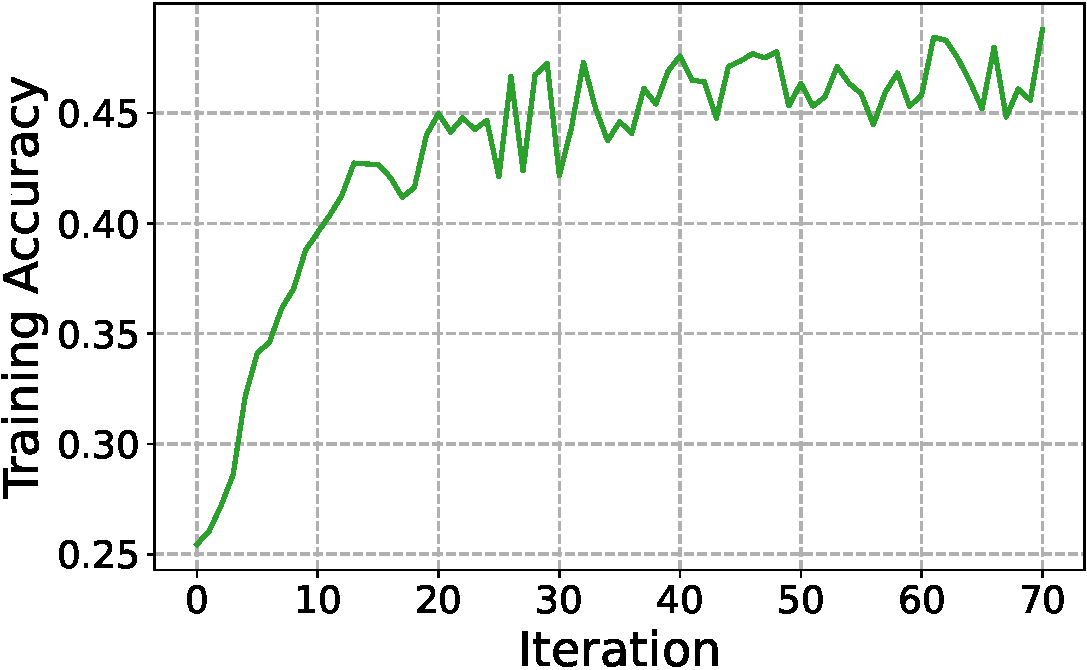
\includegraphics[width=0.87\linewidth]{figs/llama_acc.pdf}
  \end{minipage}
  \hfill
  \begin{minipage}[c]{0.32\textwidth}
    \centering
    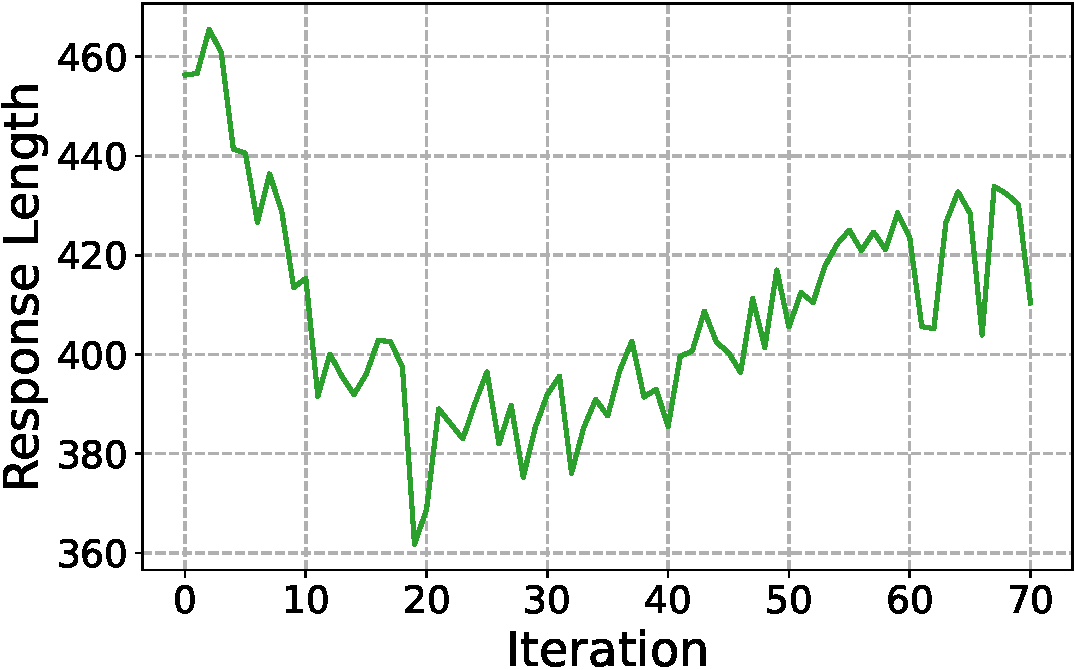
\includegraphics[width=0.87\linewidth]{figs/llama_res_len.pdf}
  \end{minipage}
  \hfill
  \begin{minipage}[c]{0.3\textwidth}
    \centering
\footnotesize
\begin{tabular}{l|l|l}
\hline
            & Base & BARL \\ \hline
GSM8K       & 69.4                  & \textbf{73.8} \\
MATH        & 47.2                  & \textbf{50.5} \\
CollegeMath & 30.8                  & \textbf{33.6} \\
Olympiad    & 16.4                  & \textbf{19.1} \\
AIME 24     & 3.3                   & \textbf{13.3} \\
AMC 23      & 27.5                  & \textbf{35.0} \\ \hline
\end{tabular}
  \end{minipage}
  \setlength{\belowcaptionskip}{-5pt}
  \caption{Results of BARL fine-tuned on Llama-3.2-3B-Instruct. \textbf{(Left)} Training accuracy and \textbf{(Middle)} response length. \textbf{(Right)} Evaluation results.}
  \label{app_fig_llama3b_res}
\end{figure}

\subsection{Token Efficiency without Greedy Decoding Outputs}\label{app_greedy}
In Figure \ref{fig_ablation_token_1}, we present the pass@k accuracies from an ablation similar to Section \ref{sec_ablation}, except that greedy decoding outputs are excluded when computing token counts and accuracies. We observe that the base and GRPO models are less robust under a sampling temperature of $1.0$, resulting in significantly lower pass@1 accuracies compared to greedy decoding. This degradation may stem from the fragility of their CoTs, which often exhibit stylistic but unproductive self-reflection and backtracking behaviors.
\begin{figure}[h]
    \centering
    \begin{minipage}[b]{0.245\linewidth}
        \centering
        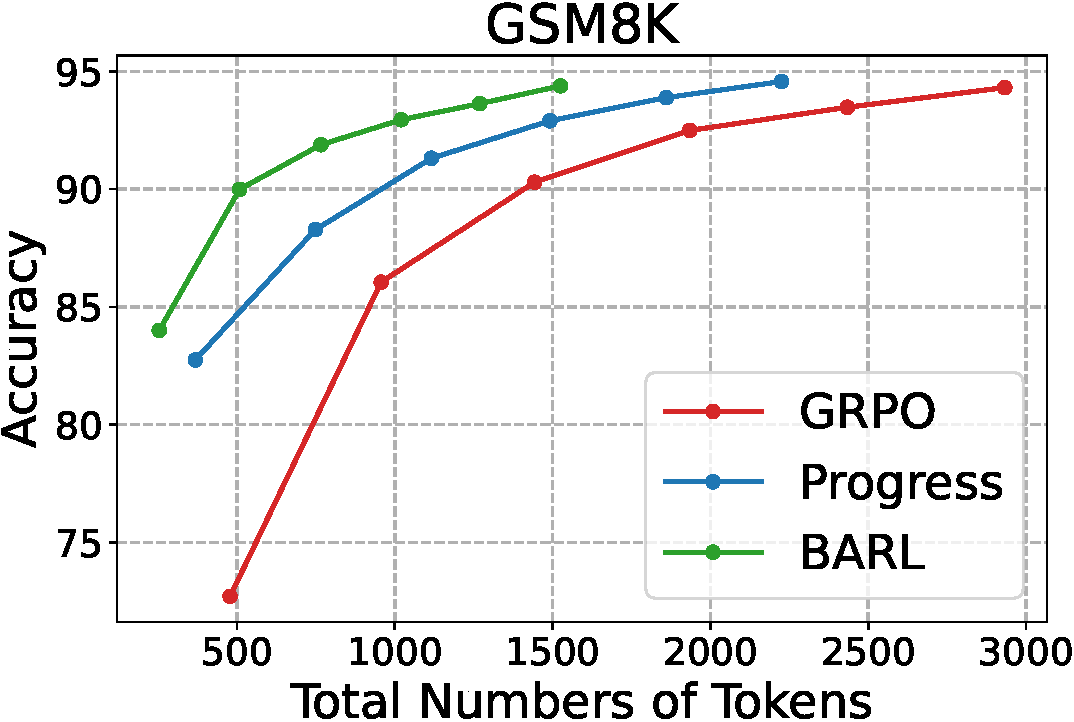
\includegraphics[width=1.023\linewidth]{figs/qwen15_gsm_token_1.pdf}
    \end{minipage}
    \begin{minipage}[b]{0.245\linewidth}
        \centering
        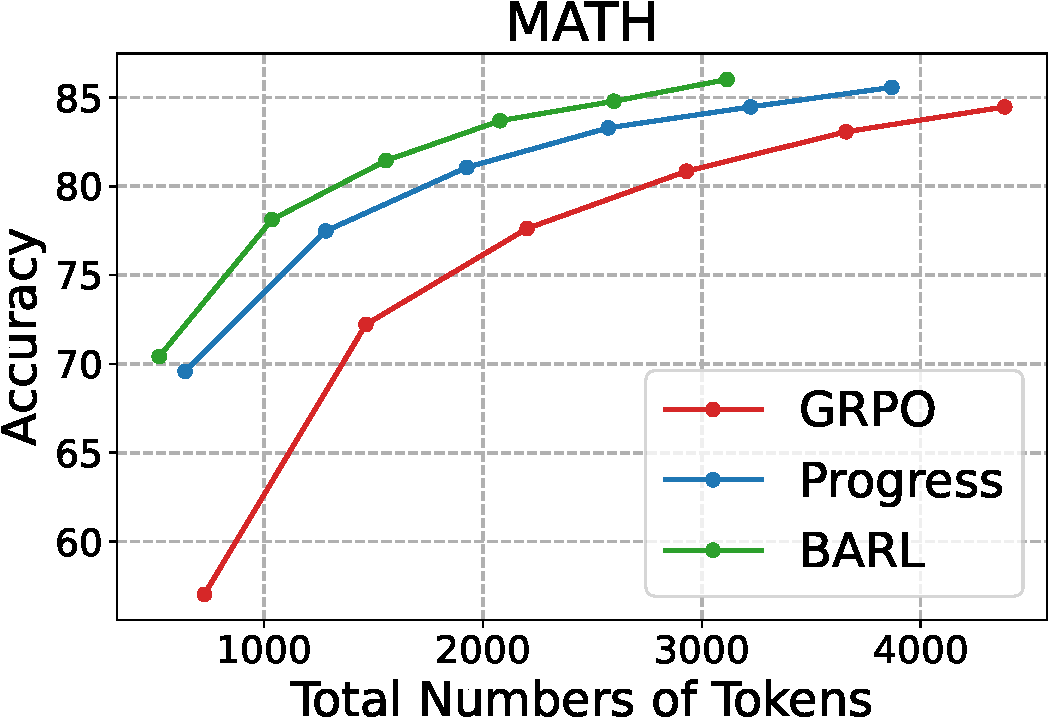
\includegraphics[width=\linewidth]{figs/qwen15_math_token_1.pdf}
    \end{minipage}
    \begin{minipage}[b]{0.245\linewidth}
        \centering
        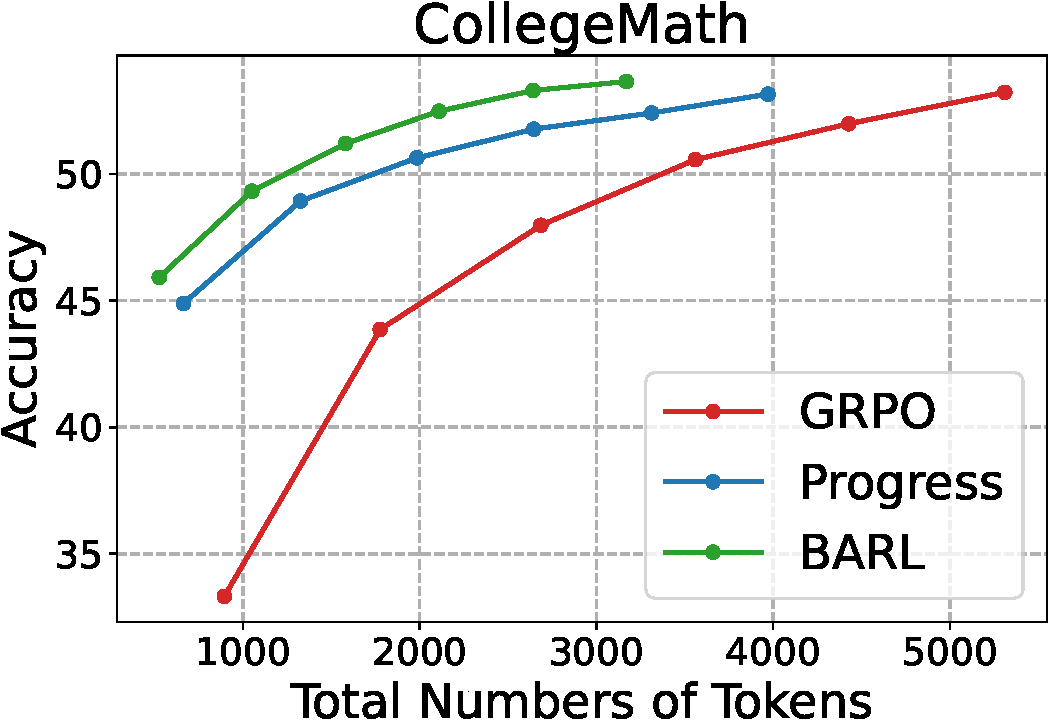
\includegraphics[width=\linewidth]{figs/qwen15_collegemath_token_1.pdf}
    \end{minipage}
        \begin{minipage}[b]{0.245\linewidth}
        \centering
    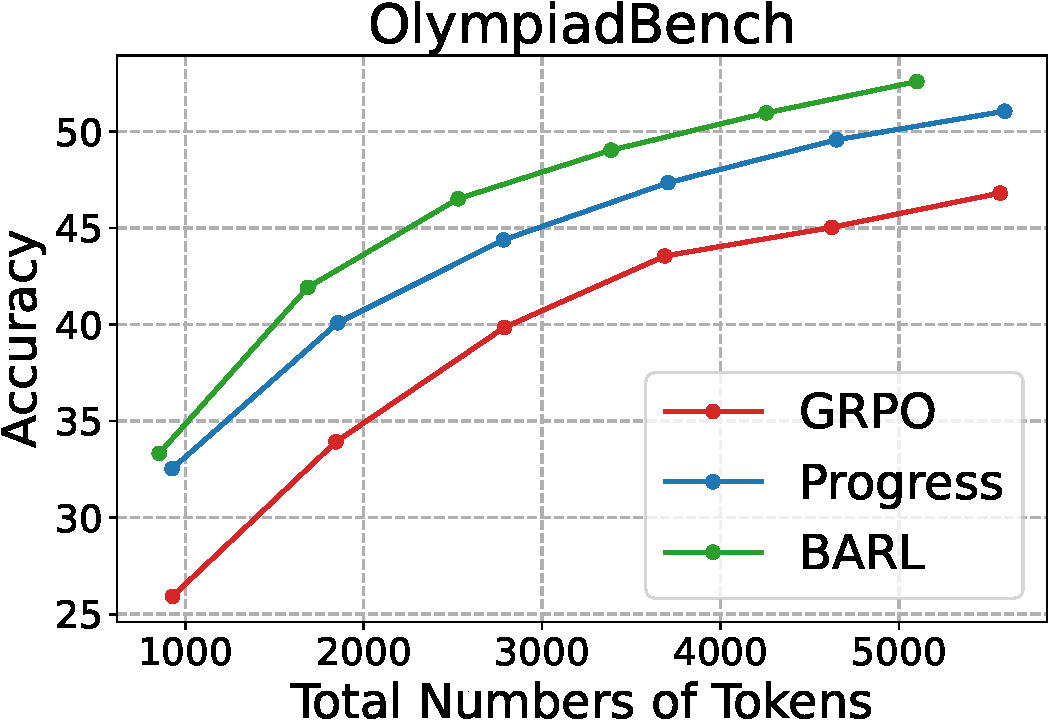
\includegraphics[width=\linewidth]{figs/qwen15_olym_token_1.pdf}
    \end{minipage}
\vspace{-0.3cm}
\setlength{\belowcaptionskip}{-10pt}
\caption{Ablation on token efficiency and pass@k accuracies with sampling temperature$=1$. GRPO and the base models are less robust to temperatures.}
\label{fig_ablation_token_1}
\end{figure}

\subsection{Some Unsuccessful Attempts}
As a straightforward implementation of the Bayes-Adaptive RL policy gradient in \eqref{eq_bayes_gradient}, we explored using value ensembles to estimate the posterior-weighted value $\EE_{\mathcal{M}\sim p(\mathcal{M}| h_t)}[Q^{\pi_\theta}_\mathcal{M}(s_t, a_t)]$. Specifically, we trained an ensemble of state-action value functions to capture epistemic uncertainty. We experimented with two approaches to constructing the ensemble: (1) fine-tuning multiple linear value heads on disjoint data subsets, each paired with chain-of-thought (CoT) trajectories and outcome rewards; and (2) applying Bayesian LoRA. However, both methods failed to effectively capture epistemic uncertainty, likely because they fine-tune only a small subset of LLM parameters, which is insufficient to fully represent the uncertainty. While maintaining independent value models may better capture this uncertainty, doing so incurs substantial computational cost. We leave the development of more efficient implementations to future work.
